\documentclass[10pt,a4paper,roman]{moderncv}
\usepackage[english]{babel}
\usepackage{graphicx}
\usepackage{pdfpages}
\usepackage{caption}
\usepackage{longtable}
\usepackage{rotating}
\captionsetup{font=footnotesize}
\newcommand{\hlbox}[1]{{\setlength{\fboxrule}{0.2pt}\setlength{\fboxsep}{2pt}\fbox{#1}}}
\moderncvstyle{classic}
\moderncvcolor{black}
\definecolor{inkblue}{HTML}{16283B}
\definecolor{steel}{HTML}{5B6B7A}
\definecolor{accent}{HTML}{8A1C2B}
\usepackage{fontspec}
\setmainfont{Latin Modern Sans}
\usepackage[scale=0.87,top=.45in,bottom=.65in,left=.80in,right=.80in]{geometry}
\usepackage{array}
\usepackage{fancyhdr}
\usepackage{lastpage}
\usepackage{setspace}
\usepackage{enumitem}
\usepackage{mdframed}
\usepackage[unicode]{hyperref}
\hypersetup{colorlinks=false, pdfborder={0 0 0}, hyperfootnotes=false}
\usepackage{titlesec}
\newcounter{legalsection}
\newcounter{legalsubsection}[legalsection]
\newcounter{legalsubsubsection}[legalsubsection]
\renewcommand{\thelegalsection}{\arabic{legalsection}}
\renewcommand{\thelegalsubsection}{\Alph{legalsubsection}}
\renewcommand{\thelegalsubsubsection}{\roman{legalsubsubsection}}

% Section: small caps, regular weight, moderately larger
\newcommand{\legalsection}[1]{%
	\refstepcounter{legalsection}%
	\par\addvspace{1.15em}%
	{\color{inkblue}\normalfont\large\scshape
		\thelegalsection.\hspace{0.55em}#1\par}%
	\vspace{0.25em}%
	{\color{inkblue}\rule{\linewidth}{0.8pt}}%
	\par\vspace{0.65em}%
}

% Subsection: small caps, bold, smaller than section
\newcommand{\legalsubsection}[1]{%
	\refstepcounter{legalsubsection}%
	\par\addvspace{0.85em}%
	{\color{inkblue}\normalfont\normalsize\bfseries\scshape
		\thelegalsubsection.\hspace{0.45em}#1\par}%
	\vspace{0.2em}%
}

% Subsubsection: small caps, regular weight, smaller still
\newcommand{\legalsubsubsection}[1]{%
	\refstepcounter{legalsubsubsection}%
	\par\addvspace{0.55em}%
	{\color{inkblue!88!black}\normalfont\small\scshape
		\thelegalsubsubsection.\hspace{0.35em}#1\par}%
	\vspace{0.1em}%
}
\pagestyle{fancy}
\fancyhf{}
\renewcommand{\headrulewidth}{0pt}
\renewcommand{\footrulewidth}{0pt}\renewcommand{\footrule}{{\color{steel}\vskip-2pt\hrule height 0.4pt}}
\fancyfoot[R]{{\color{steel}\thepage}}
\fancyfoot[L]{{\color{steel}\itshape Penn v. ODHS --- Formal Notice under Faulkner Recorded Commitment}}
\AtBeginDocument{\normalfont\normalsize}
\name{AshLe' Antoinette Penn}{}
\email{\faEnvelope\enspace \textnormal{ashlepenn.ap3@gmail.com}}
\phone[mobile]{\faPhone\enspace \textnormal{(424) 242-3374}}
\address{\textnormal{17548 NW Springville Road, Unit 9}}{\textnormal{Portland, OR 97229}}{}
\usepackage{multicol}
\newcommand{\recip}[2]{\textbf{#1}\ifx\\#2\\\else\\[1pt]{\scriptsize\itshape #2}\fi\par\medskip}
\newcommand{\figbox}[2]{{\setlength{\fboxrule}{0.3pt}\setlength{\fboxsep}{4pt}\fbox{\includegraphics[width=#1]{#2}}}}
\graphicspath{{DHS/}{./}}
\newcounter{exfigno}
\newcommand{\exfig}[3]{\par\bigskip\begin{center}%
		\hlbox{\includegraphics[width=#1]{#2}}\par\vspace{3pt}%
		\refstepcounter{exfigno}{\footnotesize\textbf{\color{inkblue}Figure \theexfigno.}~#3}%
	\end{center}\par\medskip}
\renewenvironment{quote}{%
	\par\smallskip{\color{inkblue}\rule{\linewidth}{0.7pt}}\par\vspace{6pt}%
	\leftskip1.1em\rightskip1.1em\itshape\color{inkblue!92!black}%
}{%
	\par\vspace{6pt}{\color{inkblue}\rule{\linewidth}{0.7pt}}\par\smallskip%
}
\setlength{\parindent}{0pt}
\setlength{\parskip}{\baselineskip}
\begin{document}
	
	{\color{inkblue}\noindent\rule{\textwidth}{1.3pt}}
	\vspace{0.35em}
	
	\begin{center}
		{\color{inkblue}\textbf{In the Matter of A.\,D., Washington County Circuit Court No.~25JU04261}}\\
		\small \textit{Formal Notice of Fabrication, Material Omission, and Required Action}\\
		\small \textit{Delivered Under the Standard the Recipient Bound Themselves to During January 28, 2026 Recorded Commitment}
	\end{center}
	
	\begin{flushright}
		\textbf{AshLe' Penn}\\
		\scriptsize{17548 NW Springville Road, Unit 9}\\
		\scriptsize{Portland, OR 97229}\\
		\scriptsize{\faPhone\enspace (424) 242-3374}\\
		\scriptsize{\faEnvelope\enspace ashlepenn.ap3@gmail.com}
	\end{flushright}
	
	\vspace{0.8em}
	
	\noindent\textbf{To:}\par\smallskip
	{\raggedright\recip{Sonya Faulkner}{D16 Manager, Oregon Department of Human Services --- Child Welfare\\ Sonya.Faulkner@odhs.oregon.gov}}
	
	\noindent\textbf{Cc:}\par
	\setlength{\columnsep}{1.5em}
	\begin{multicols}{2}
		\raggedright\setlength{\parindent}{0pt}
		\recip{Yazmin Wadia --- Assistant Attorney General}{yazmin.wadia@doj.oregon.gov}
		\recip{Laurie K.~Hernandez --- Child Welfare Program Manager}{laurie.k.hernandez@odhs.oregon.gov}
		\recip{Alicia L.~Reynolds --- Child Welfare Manager}{alicia.l.reynolds@odhs.oregon.gov}
		\recip{David Milne --- Social Service Specialist}{david.milne@odhs.oregon.gov}
		\recip{Skye F.~Hopkins --- Resource Developer}{skye.f.hopkins@odhs.oregon.gov}
		\columnbreak
		\recip{Kimberly Beck --- Juvenile Processing Clerk}{kimberly.a.beck@ojd.state.or.us}
		\recip{Richard Moellmer --- Trial Court Administrator}{richard.e.moellmer@ojd.state.or.us}
		\recip{Fariborz Pakseresht --- Director, ODHS}{}
		\recip{Rolanda Garcia--- Interim Director, ODHS Child Welfare Division}{}
		\recip{Oregon Attorney General}{attorneygeneral@doj.oregon.gov}
		\recip{Oregon Foster Care Ombudsperson}{alexis.l.amorelli@odhs.oregon.gov}
		\recip{Office of Washington County Counsel --- }{countycounsel@washingtoncountyor.gov}
	\end{multicols}
	\vspace{1.0em}
	\normalsize
	\begin{center}
		\textbf{Enclosed Records (Exhibits A through S)}
	\end{center}
	\begin{enumerate}[label=\textbf{Exhibit \Alph*.},leftmargin=*,itemsep=0.2em,topsep=0.2em]
		\item Neuropsychological Evaluation / Parental Assessment of AshLe' Penn by Christopher K.~Tongue, Ph.D., Licensed Psychologist (evaluation date 10/30/2021).
		\item Letter from Al-Quan Davis to AshLe' Penn dated January 15, 2023 (Alquan\_Davis\_2023.pdf).
		\item Audio excerpt of Sonya Faulkner's January 28, 2026 statement (Sonya\_Faulkner\_Byte.mp4).
		\item Audio recordings of January 28, 2026 and April 28, 2026 recorded calls (recantation and no-parental-capacity-assessment admissions).
		\item Kimberly Beck email of September 9, 2025 at 3:09 PM rejecting Mother's September 8, 2025 filing.
		\item Full October 31, 2025 jurisdictional trial transcript (Emilie Marquand testimony; Judge Rini rulings).
		\item Rylan Duffy \emph{Declaration of Diligent Efforts toward Service} (October 10, 2025).
		\item Kayla Miller \emph{Affidavit Regarding Efforts to Serve Parent} (October 28, 2025).
		\item Sonya Faulkner emails of June 2, 2026 (10:33 AM and 3:19 PM).
		\item Copy of Notice of Tort Claim and § 1983 Pre-Suit Demand.
		\item Washington County HR fee-waiver denial letter from Aaron Mendes dated September 19, 2025 (referencing ``evidence the County has in its possession'').
		\item Washington County District Attorney's October 31, 2025 denial opinion signed by Deputy DA Sabina Khachaturova.
		\item Petitioner's October 17, 2025 Petition for Review of Fee Waiver Denials served on DA Barton.
		\item Text-message thread from ODHS Supervisor Heather Kitto documenting the 5:40~PM September~6, 2025 release text and the 5:59~PM reversal text (19-minute reversal window).
		\item Shelter Hearing transcript excerpts (September 8, 2025) confirming Mother's telephonic contact with the court and the unauthorized appearance of attorney Ireland Mahoney.
		\item ODHS records reflecting the 3/26/2024 two-hour in-home interview at Mother's residence and the ``Out of control not believed to be met'' supervisor consultation finding.
		\item ARIA certification of completion of mental health services as directed by the court.
		\item Wolfpack Consulting and Therapeutic Services, LLC Progress Notes (Partial Records to establish participation - not disclose confidential information.)
		\item Mother's early attempts to resolve any services required, it would take the agency YEARS to establish the "treatment" it relied so heavily on as a barrier to return
	\end{enumerate}
	
	\bigskip
	\begin{center}
		\noindent\textbf{RE: False Testimony, Material Omission/Selective Reporting, and Fabricated Evidence by ODHS Staff in \textit{In re A.D.}, Case No.~25JU04261;
			Required Action Under Your Recorded Commitment of January 28, 2026}\\
		\textit{Sent by Email With Enclosed Recordings, Court Transcript, and Exhibits A through S}\\
		\textit{Proposed Stipulation Attached as Appendix A}
	\end{center}
	
	\vspace{1.0em}
	
	Ms.~Faulkner,\\
	
	\noindent``Parents and children have a well-elaborated constitutional right to live together without governmental interference. That right is an essential liberty interest protected by the Fourteenth Amendment's guarantee that parents and children will not be separated by the state without due process of law except in an emergency.'' \emph{Wallis v.~Spencer}, 202 F.3d 1126, 1136 (9th Cir.~2000). My family has been subjected to precisely the form of state interference the Ninth Circuit forbids. Al-mira's removal was based on an insufficient investigation, the repeated suppression of exculpatory facts, social workers' intentional misrepresentations of agency action, and a fabricated narrative about my family delivered to the court with knowledge of the truth.\\
	
	\noindent The Ninth Circuit has addressed the precise constitutional injury that occurs when social workers lie to a dependency court in order to separate a parent and child. In \emph{Hardwick v.~County of Orange}, social workers told the dependency court that the mother had caused her daughters to miss a mandatory visit with their father, when the actual problem had been caused by the visitation monitor. The social workers further represented that the mother had turned the children against the monitor and had told them that their father was trying to take them away. The record showed that the social worker herself had made the inappropriate and threatening statements to the children. On the basis of those false representations, the dependency court concluded that the mother was ``using'' her children and immediately removed the girls from her custody. \emph{Hardwick v.~County of Orange}, 844 F.3d 1112, 1117--19 (9th Cir.~2017).\\
	
	\noindent That is not a distant or abstract comparison. It is the same constitutional mechanism used here: ODHS social workers supplied the court with false accounts of my conduct, concealed or omitted the facts that contradicted those accounts, converted my efforts to protect my daughter and obtain information into evidence against me, and then relied on the resulting false narrative to establish jurisdiction, obtain default findings, keep Al-mira separated from me, and impose services upon me. ODHS also retaliated against me for exercising my right to decline voluntary, non-court-ordered engagement with the agency. Rather than acknowledge that I retained the right to demand a lawful basis for agency intervention, to communicate in writing, to decline unrequested services, and to withhold consent to agency demands not ordered by a court, ODHS portrayed my exercise of those rights as ``non-engagement,'' ``refusal,'' ``lack of cooperation,'' and evidence that I was unwilling or unable to protect my daughter.\\
	
	\noindent In \emph{Hardwick}, the Ninth Circuit held that social workers were not entitled to absolute immunity for alleged fabrication of evidence, perjured testimony, and false representations made outside their legitimate quasi-prosecutorial role. The court further held that deliberate fabrication and use of false evidence to separate a parent from her children violates clearly established constitutional rights and is not protected by even qualified immunity. \emph{Hardwick}, 844 F.3d at 1118--23.\\
	
	\noindent This is what happened here. Emilie Marquand lied under oath. She gave the court factual assertions that were false, contradicted by ODHS's own records, contradicted by her own testimony in the same period of testifying, or made without \textit{any} evidentiary support. Those lies were material. The court relied on these fabricated or misleading characterizations and has since treated me as if I have abandoned my daughter and offended the court. The truth of the matter is that ODHS has absolutely no evidence of \textit{any history} that I have abused/neglected my daughter, no evidence that I have ever used their father or his home as punishment, no evidence that I refused to retrieve my daughter from the hospital, no evidence that my own Mother believes me to be unfit or that she's attempted to gain custody of my children, no evidence that the agency removed her from my care on September 6, 2025 under a lawful basis, no evidence that Al-mira is unsafe in my home with the last worker to have assessed my home finding the exact opposite (the only narrative that she is unsafe has come from ODHS workers who \textbf{have not} assessed my home), no evidence that I am unable/unwilling to understand the needs of my child (with the only clinical assessment in the record coming from a \textit{qualified individual} by Dr. Tongue), no evidence that I do not engage substantially in services during a prior period of your agency's interference in my home, no evidence that the agency notified me of the date/time of the shelter hearing to support its claims of my avoidance --- Ms. Faulkner, the list could continue. \\
	
	\noindent The following are the specific lies, fabrications, omissions, and material misrepresentations ODHS presented to the court through Marquand's sworn testimony:
	\begin{enumerate}[label=\arabic*., leftmargin=0.5in, itemsep=0.85em]
		
		\item \textbf{Marquand testified that I ``did not engage in any services'' and ``failed to do any of the services'' in the prior dependency case.} She specifically identified parenting classes, stable housing, visitation, a neuropsychological evaluation, agency contact, victim/survivor services, releases of information, and participation in the children's services. That testimony is false. The agency possessed records showing, among other things, my completed neuropsychological evaluation with Dr.~Tongue, parenting education, domestic-violence services, signed releases, agency contacts, and my self-initiated domestic-violence grant. The blanket assertion that I completed \emph{none} of those services was not a reasonable characterization of the record; it was a material fabrication.
		
		\item \textbf{Marquand then contradicted her own ``no engagement'' testimony.} In the same hearing, when discussing the twenty hotline calls related to Father, she testified that I had engaged in those assessments---then changed that to say that I had engaged ``limitedly.'' ODHS cannot truthfully tell the court, on the one hand, that I did not engage in \emph{any} services and, on the other, that I engaged in the assessments but only ``limitedly.'' The first statement was used to portray me as wholly noncompliant; the latter confirms that the first was false.
		
		\item \textbf{Marquand testified that I \underline{refused} to pick Al-mira up from the hospital and \underline{refused} to protect her.} That statement omits the actual circumstances and recasts my demand for an explanation of ODHS's claimed authority as parental abandonment. The agency contacted me after Al-mira had already been taken into protective custody; I demanded that ODHS explain the basis for continuing custody once I had been reached. I also arranged for her maternal great-uncle to go to the hospital at my request as he could reach her more immediately and thereby return her to my care much faster. The agency's own report confirms that he arrived at the hospital at my request. My insistence that ODHS articulate a lawful basis for continued custody is not evidence that I refused to protect or retrieve my child.
		
		\item \textbf{Marquand presented speculation that I ``coached'' Al-mira to recant as though it were an established fact.} The actual record reflects that Al-mira told the agency that ODHS had lied to me about what she said and that she had not made the statement attributed to her. Marquand converted that denial into an accusation that I coached my daughter, without identifying any direct evidence that I coached her and despite the absence of any finding establishing that accusation. Speculation from a hospital social worker or agency employee is not evidence that a mother coached her child. Marquand nevertheless presented that accusation under oath as part of the factual basis for jurisdiction. The accusation was false, defamatory in its ordinary meaning, unsupported by evidence, and materially prejudicial because it portrayed Mother as manipulating her daughter, undermining Al-mira's credibility, and interfering with the agency's ability to assess safety. It then became part of the official agency and court record used to justify continued separation.
		
		\item \textbf{Marquand used ``32 calls'' to create a false narrative of substantiated abuse, neglect, physical abuse, and substance use by Mother.} She testified that the calls concerned neglect, threat of harm, exposure to violence, physical abuse, and substance use. But a hotline call is not a founded finding. The number of calls cannot be presented as proof that their allegations were true, and the number attributed to Mother is severely misrepresented, as demonstrated below. The agency's own disposition history distinguishes founded, unfounded, unable-to-determine, screened-out, duplicate, and pending matters. Aggregating all calls into a single adverse ``history'' was materially misleading and an omission of the truth used to mislead the court.
		
		\item \textbf{Marquand invoked substance use while admitting that ODHS had not assessed it.} She testified that there were ``significant concerns around the substance use,'' but immediately admitted that the cases were pending and that ODHS had not had meaningful contact with me ``to fully assess \ldots and get information about her substance use.'' ODHS presented substance use as a \emph{concern}---which does not meet the threshold for emergency protective custody---in support of jurisdiction while admitting it had not obtained the information necessary to establish whether substance use existed, whether it affected parenting, or whether it posed any danger to Al-mira.
		
		\item \textbf{Marquand testified that I failed to protect Al-mira from Father while omitting ODHS's own role in treating Father as a safe placement.} ODHS endorsed Father as a safe placement and participated in lifting the no-contact barrier after his first arrest and after Al-mira had been placed with me successfully for several months. It was ODHS that allowed Al-mira's return to Father's care, and Marquand's testimony failed to mention the assessments that occurred after her placement with me, that there were no concerns for her while in my care, and that the agency itself knew of the escalations and documented the need to act but did not. Instead, the agency advocated for removal of the no-contact order, which would lead to the later assault and strangulation allegations arising after Al-mira was back in Father's care. ODHS cannot place a child with Father, characterize Father as safe, and then use the resulting danger as proof that Mother failed to protect her from the very placement ODHS endorsed --- all while omitting Mother's assessments and engagement, and while testifying that Mother had not engaged whatsoever.
		
		\item \textbf{Marquand faulted me for failing to modify the domestic-relations custody order while omitting the procedural and jurisdictional barriers to doing so.} She presented Father's sole custody as though it established my inability or unwillingness to protect Al-mira, without identifying any lawful mechanism available to me to unilaterally alter Father's custody order, and without acknowledging the jurisdictional barriers that prevented me from obtaining the relief ODHS now says I should have secured. She omitted that Al-mira was \emph{safely} placed with me, enrolled in school, and \textbf{evaluated and assessed \underline{within} my home}. She also omitted that I submitted a request to Washington County Circuit Court to modify custody, but the court declined to accept it because it determined it lacked jurisdiction at the time of filing.
		
		\item \textbf{Marquand testified that I made ``very little'' meaningful attempt at visitation while ODHS had not provided a workable visitation plan.} ODHS failed to substantiate the authority it claims it had when it exercised emergency protective custody on 9/6/25, and Marquand's testimony attributed visitation failures to me. Marquand failed to inform the court that Al-mira's placement was more than thirty miles away, required several hours of bus travel, and that I lacked transportation. ODHS provided no assistance in facilitating visitation. The agency restricted my contact with her while she was hospitalized without identifying what harm it claimed to be preventing, then delayed or withheld a concrete visitation structure and treated the predictable absence of agency-facilitated visits as evidence against me. ODHS cannot withhold a plan, restrict contact, provide no transportation support, and then characterize the resulting lack of visits as Mother's lack of interest in her child. Further, DHS policy requires first visit within a week and encourages caseworkers to schedule first visit within 48 hours - as stated by the court at the shelter hearing. ODHS did not fulfill this requirement and would then later attribute its failings to adhere to its own rules on me. 
		
		\item \textbf{Marquand characterized my emails as ``more demands than anything.''} My written communications sought the factual basis for ODHS's actions, its position on the authority it claimed to be exercising over the emergency removal, information about my daughter, the records necessary to understand the allegations, and documented communication with a system I have---especially now---proven reasons not to trust. Calling those requests ``demands'' reframed my efforts to obtain information I am entitled to and to protect my legal relationship with my daughter as proof of non-engagement. It was designed to punish me for requesting accountability rather than evidence that I failed to parent or protect Al-mira.
		
		\item \textbf{Marquand testified that Al-mira did not want to return to Mother, while later acknowledging that Al-mira was willing and wanting to live with Mother after family counseling.} Those statements cannot both be presented as a categorical basis for continued separation. The latter testimony confirms that Al-mira's position was not an absolute rejection of Mother, but a desire for support and counseling in restoring the relationship. This testimony also disregards several documented statements from my daughters describing their relationship with me to the contrary.
		
	\end{enumerate}
	
	\noindent Ms.~Faulkner, these are some of the representations that ODHS placed before the court while I was denied notice (Al-mira's lawyer states in a letter to her that the agency attempted to serve me between 9/30/25 and 10/14/25 --- nearly a month after her removal; this is not acceptable for an agency that claims that I refused to appear), the petition, the reports, the evidence, and a genuine opportunity to respond and defend. The defective service and default process did not merely create a procedural problem. It enabled these assertions to be presented without contradiction, testing, cross-examination, or correction, and then converted into jurisdictional findings against me. The agency had knowledge that, and certified in its Declaration of Diligent Efforts, the earliest attempts at service took place on October 10, 2025 - well after Al-mira's removal. This does not afford a parent an opportunity to appear and defend at the shelter hearing as required by ORS 419B.185(1). The agency also had knowledge that it sent its process server to an incorrect address (conceded on the record in open court at a later hearing) yet did not move to correct the diligent efforts assertions it had already made. \\
	
	Even more to this point, ODHS possessed and used language drawn directly from the court-ordered neuropsychological evaluation I completed during prior involvement with your agency, yet it mischaracterized the extent of my participation and portrayed me to the court as a parent who had failed to engage or complete services. It then tried to recast that prior history as evidence of a purported ``pattern'' in the present proceeding, even though the record does not support that characterization \textbf{and} the agency is required to provide \underline{current} proof of a non-speculative and serious threat likely to be realized.\\
	
	Marquand's testimony identified \textit{nothing} demonstrating that any threat to Al-mira was current, likely to be realized, or that threatened serious loss or injury. The testimony represented generalizations, speculation, and outright falsifications of factual information (as with the purpose of outstanding warrants and substance abuse that has \textbf{never} been established by your agency). ODHS also attributed at least two statements to my mother that she has now sworn, under oath, were never made. These are not harmless errors; they are knowing or reckless misrepresentations that foreseeably injure both parent and family. No good-faith defense can excuse falsifying a parent's history to mislead the court or inventing statements and attributing them to that parent's mother. For that reason, neither absolute nor qualified immunity should be understood to shield ODHS personnel from liability for this conduct.\\
	
	On our recorded call of January 28, 2026, you stated\footnote{See SonyaFaulknerByte.mp4.}:
	
	\begin{center}
		\begin{minipage}{0.80\textwidth}
			\begin{quote}
				\textit{If I were to find any unlawful or concerning information in the record or any information that we perjured ourselves, I would absolutely handle that with our employees and also notify the court.}
			\end{quote}
		\end{minipage}
	\end{center}
	
	\vspace{1em}
	You added that you would review the representations at issue and reconnect. In subsequent calls and emails, however, you did not engage the substance of those concerns or obtain access to the underlying records. You repeatedly pointed to the fact that the juvenile court had already taken jurisdiction, as though the existence of a jurisdictional finding were itself an answer to my claim that \textbf{ODHS obtained jurisdiction by presenting fabricated and misleading evidence and omitting the truth}. Jurisdiction entered on the basis of false evidence is not self-justifying; it is the core of the due process violation I have been describing.
	
	\legalsection{Emergency Protective Custody Was Taken on a Basis the Agency Never Authorized, Never Pleaded, and Never Placed Before Any Court}
	
	\noindent The standard governing an emergency removal without a court order is not merely whether a child’s circumstances appear concerning. Before January 1, 2020, ORS 419B.150 permitted removal when a child’s ``condition or surroundings reasonably appear to be such as to jeopardize the child’s welfare.'' The Oregon Judicial Department recognized that this earlier standard was insufficient under federal and state constitutional law because the Fourth and Fourteenth Amendments require both exigency and severe harm before the State may separate a child from a parent without prior judicial authorization.\\
	
	\noindent Effective January 1, 2020, House Bill 2849 removed that welfare-jeopardy language. ORS 419B.150 now permits protective custody without a court order only when there is reasonable cause to believe that: (1) the child faces an imminent threat of severe harm; (2) the child poses an imminent threat of severe harm to self or others; or (3) the parent or guardian will imminently cause the child to be beyond the juvenile court’s reach before a court order can be obtained. ORS 419B.150(4)(a). ``Severe harm'' means life-threatening damage or a significant or acute injury to a person's physical, sexual, or psychological functioning. ORS 419B.150(3)(c).\\
	
	\noindent ODHS therefore had to identify which statutory emergency predicate authorized taking Al-mira without a court order, the specific facts supporting that predicate, and why immediate custody---rather than release to Mother, a safety plan, medical treatment, relative support, transportation assistance, or another less restrictive measure---was necessary to prevent the identified imminent severe harm. The agency did none of those things.\\
	
	The protective-custody report describes the immediate event as an alleged violent incident between Al-mira and her father, his arrest, and the child's hospital evaluation. As to Mother, the report largely moves from statements such as ``not open to engaging,'' inability to ``fully assess,'' and generalized historical concerns to conclusory assertions that Mother lacked skills, would not protect Al-mira, and had criminal activity interfering with parenting. That distinction is crucial:
	
	\begin{center}
		\renewcommand{\arraystretch}{.90}
		\begin{tabular}{@{}p{0.43\textwidth}@{\hspace{9pt}}p{0.43\textwidth}@{}}
			\hline
			\textbf{What ODHS needed to establish} &
			\textbf{What the record does not establish} \\
			\hline
			A present safety threat specifically tied to Mother &
			Specific conduct by Mother creating a current, non-speculative danger to Almira. \\
			\hline
			Why removal from Mother's care was necessary &
			A factual explanation of why Almira could not safely be released to Mother, with protective conditions or safeguards if needed. \\
			\hline
			Why less restrictive alternatives would not protect Almira &
			An analysis of placement with Mother, supervision, transportation assistance, safety planning, relative support, or other protective measures. \\
			\hline
			A meaningful opportunity for Mother to contest the allegations &
			Valid service; access to the petition, reports, and evidence; and a meaningful opportunity to appear, prepare, respond, and present evidence. \\
			\hline
		\end{tabular}
	\end{center}
	
	\legalsubsection{The agency told Mother the reason for custody, in writing, at the moment it decided: the child's self-harm statement --- nothing about Mother's conduct.}
	At 5:40 PM on September 6, 2025, ODHS Supervisor Heather Kitto texted Mother: ``we can release custody to you.'' Nineteen minutes later, at 5:59 PM, Kitto reversed that decision in writing: ``We've received new information that your child has disclosed suicidal intent if she was made to return to your care, so she will remain in protective custody while we assess these concerns.'' Kitto's contemporaneous email states the same basis, and worker Bennett's note identifies ``the high risk note for suicidal ideation'' as the reason ``the agency would maintain Protective Custody and request a Shelter Hearing.'' The stated basis was the child's self-harm risk --- not Mother's conduct, and not any deficit in Mother's parenting capacity.\footnote{\textit{Record cite:} Notice of Tort Claim p.~4 (Kitto texts); 2025-10-07 ODHS Report p.~2 (Kitto email); 2025-09-08 Protective Custody Report pp.~5, 7.}\\
	\par\bigskip
	\begin{center}
		\begin{minipage}[c]{0.30\textwidth}\centering\hlbox{\includegraphics[height=3.5in]{kitto.png}}\end{minipage}\hfill%
		\begin{minipage}[c]{0.05\textwidth}\centering{\color{accent}\Large$\longleftrightarrow$}\end{minipage}\hfill%
		\begin{minipage}[c]{0.27\textwidth}\centering\hlbox{\includegraphics[height=3.5in]{FirstNoticePCStamped.png}}\end{minipage}\hfill%
		\begin{minipage}[c]{0.05\textwidth}\centering{\color{accent}\Large$\longleftrightarrow$}\\[3pt]{\footnotesize\color{accent}\textbf{19 min}}\end{minipage}\hfill%
		\begin{minipage}[c]{0.27\textwidth}\centering\hlbox{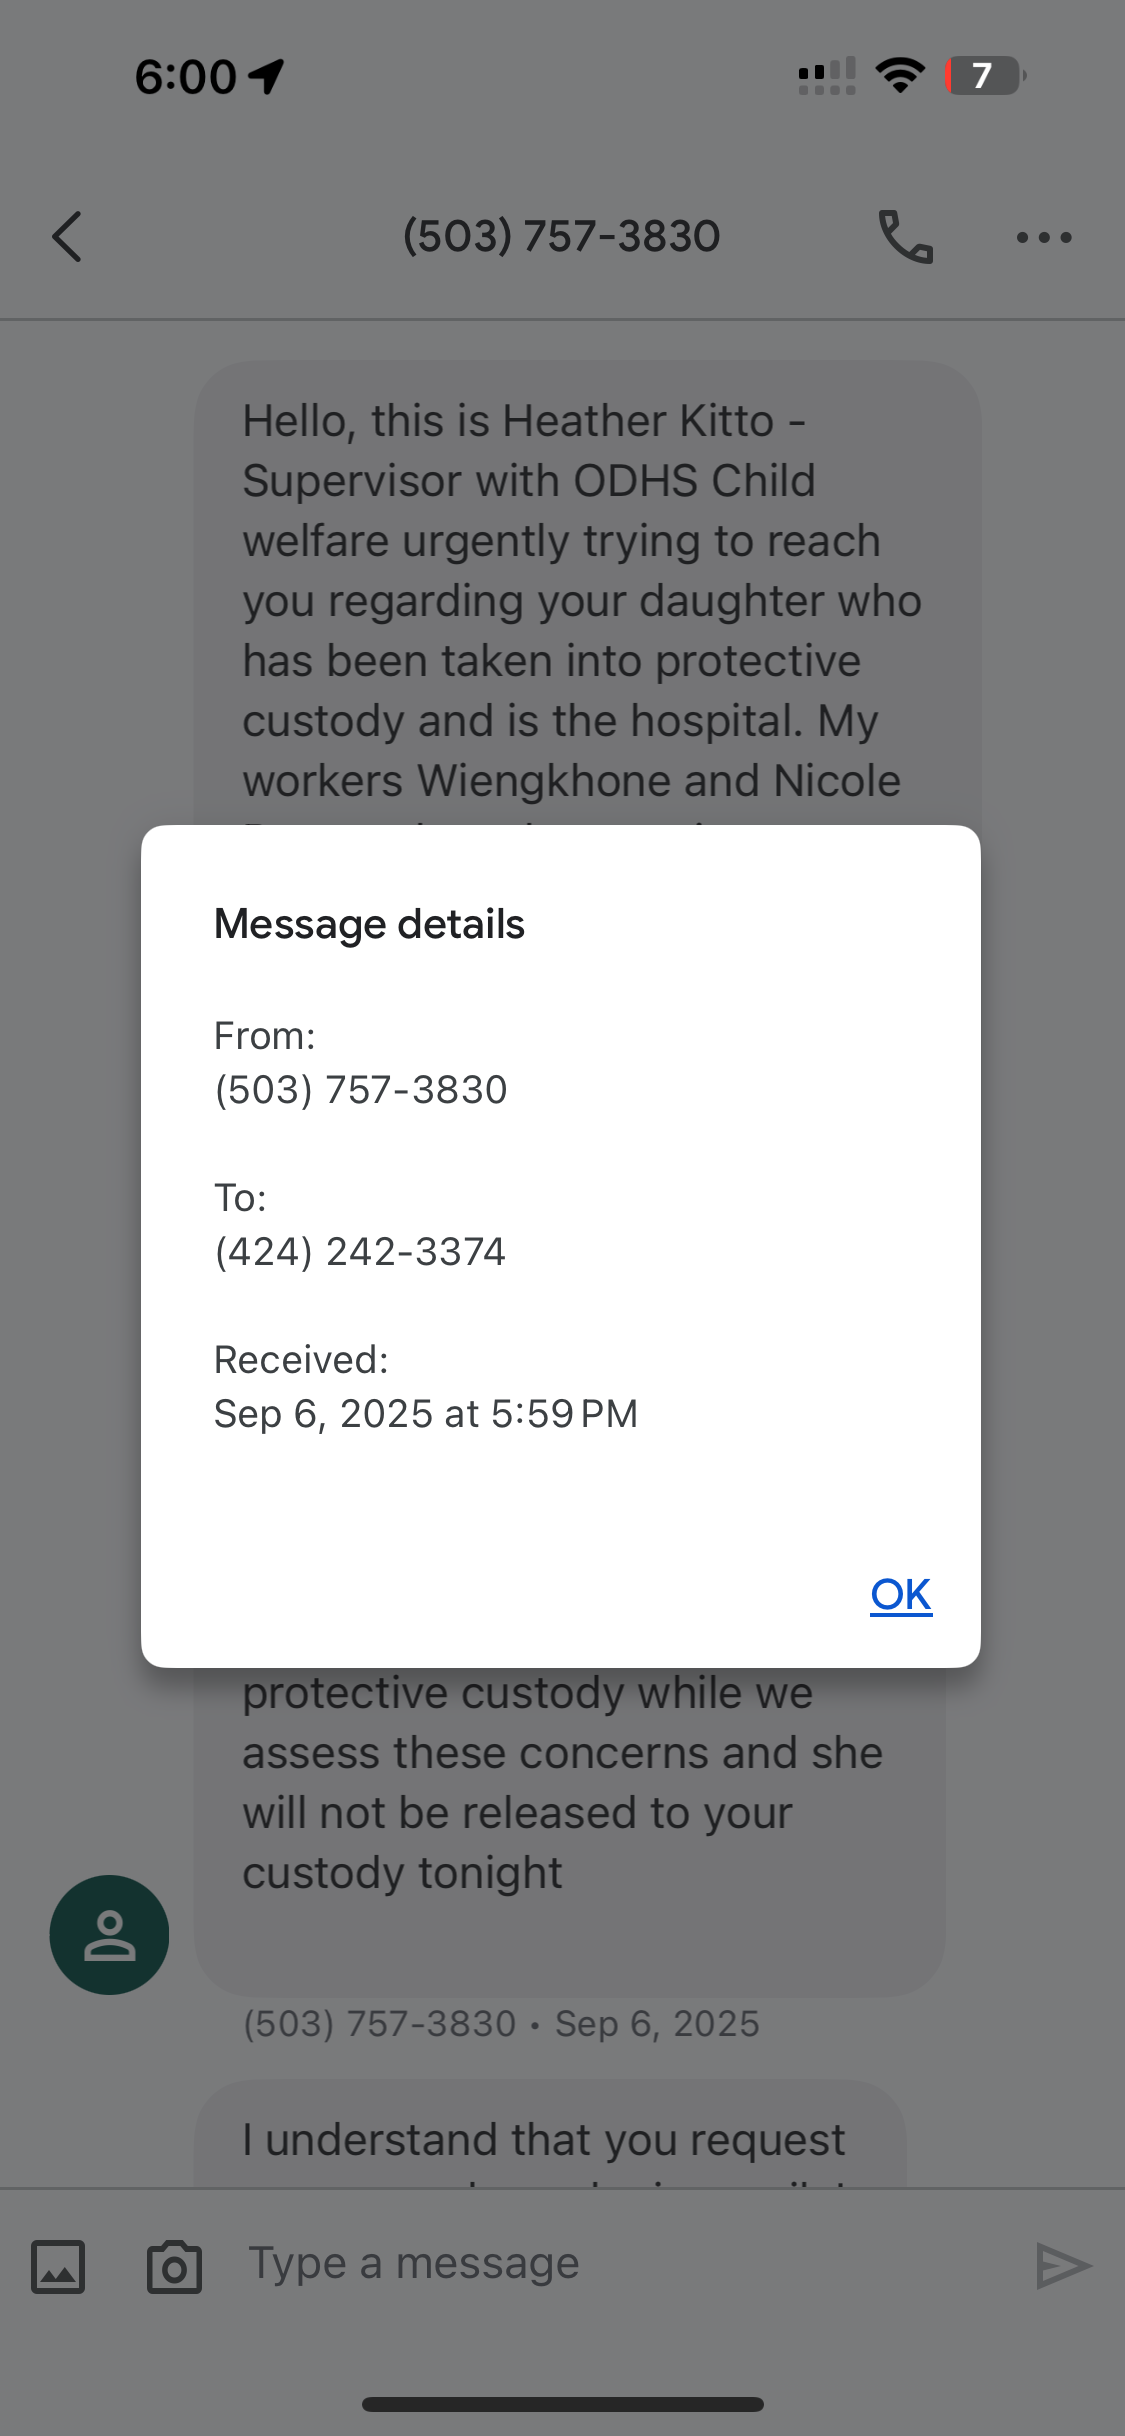
\includegraphics[height=3.5in]{SecondNoticePCStamped.png}}\end{minipage}%
		\par\vspace{6pt}
		\refstepcounter{exfigno}{\footnotesize\textbf{\color{inkblue}Figure \theexfigno.} The nineteen-minute reversal, in the agency's own metadata. \textbf{Left:} the full text thread. \textbf{Center:} 5:40~PM, September~6, 2025 --- ``we can release custody to you.'' \textbf{Right:} 5:59~PM --- the child ``has disclosed suicidal intent if she was made to return to your care, so she will remain in protective custody.'' The reason ODHS gave Mother, in writing, is the child's self-harm disclosure; the agency states no deficit in Mother's parenting and identifies no dangerous act by Mother. \textit{(Source: Kitto text messages; carrier message-details timestamps.)}}
	\end{center}
	\par\medskip
	
	\legalsubsection{The agency told Mother a summons would be delivered --- it never told her the hearing's date or time.}
	Across the emails and calls ODHS exchanged with Mother on September~6, 7, and 8, 2025, no worker gave Mother the date or the time of the shelter hearing. Kitto's written notice states only that ``a worker will be coming to your home today with the court summons.'' Mother received no hearing date, no time, and no appearance instruction. The promised summons is the sole reference to court process in the agency's contemporaneous communications, and the record does not establish that any summons was in fact delivered to Mother before the September~8 hearing. A parent cannot be treated as having declined to appear at a hearing whose date and time the agency never disclosed.\footnote{\textit{Record cite:} Kitto text message, September~7, 2025; see also the service defects catalogued below.}
	
	\exfig{0.30\textwidth}{KittoNOTNoticeOfHearing.png}{The only message in the record touching court process: ``a worker will be coming to your home today with the court summons.'' No hearing date or time is given. The same message confirms ODHS was placing the child with the maternal relative (``Mark'') and certifying him as a foster parent. \textit{(Source: Kitto text message, September~7, 2025.)}}
	
	\legalsubsection{The agency's own ORS 419B.171 form has a box for exactly that basis --- and the agency did not check it.}
	The Protective Custody Report form directs the agency to mark the statutory predicate: (A)~protect from abuse; (B)~prevent the child from inflicting harm on self or others; (C)~keep the child within reach of the court; (D)~ICWA; (E)~medical assessment of suspicious injuries. Option~B is the self-harm predicate --- the exact circumstance Kitto described. \textbf{The agency did not select it.} The Shelter Order entered September 8, 2025 instead marks that the child could not be safely returned without danger of ``suffering physical injury or emotional harm'' and ``not remaining within the reach of the court.'' The agency removed on a self-harm rationale and then recorded the removal on grounds of \emph{parental} harm and flight risk. The predicate it told Mother about is not the predicate it certified to the court.\footnote{\textit{Record cite:} 2025-09-08 Protective Custody Report p.~2; 2025-09-08 Shelter Order p.~3, \S 6.}
	
	\legalsubsection{The self-harm basis was never pleaded as a jurisdictional allegation.}
	The three allegations found proven against Mother on October 31, 2025 are (A)~lack of understanding/skills, (B)~failure to protect from Father, and (C)~criminal activity. None is the reason the agency gave Mother for taking her daughter. The self-harm statement --- the operative emergency predicate, communicated in writing at 5:59 PM on September~6 --- was never pleaded as a jurisdictional basis at all. It was never subjected to adversarial testing because it was never pleaded.\footnote{\textit{Record cite:} 2025-09-08 Protective Custody Report pp.~3, 9; Notice of Tort Claim p.~8.}
	
	\legalsubsection{The statement was recanted, and the agency knew it before the shelter hearing.}
	The attributed statement was that the child ``would attempt suicide if she went home with her mom.'' Hospital social worker Leah Sathrum --- the source of that attribution --- documented that the account ``was definitely not what child said initially'' and that she was ``worried the change in statements was due to parents' reaction.'' The child recanted to Sathrum and to Mother directly; both Sathrum and ODHS worker Bennett recorded the recantation. It appears \emph{nowhere} in the September~8 shelter petition, the Shelter Order, or the diligent-efforts submissions. The agency held the exculpatory fact and withheld it from the court deciding whether to continue custody.\footnote{\textit{Record cite:} 2025-10-23 ODHS Report pp.~12, 22--23; Notice of Tort Claim p.~4.}
	
	\legalsubsection{You have already acknowledged the defect, on a recorded call.}
	On our January~28, 2026 recorded call you acknowledged the recantation (19:18: ``once there was a recantation for that to be considered''). That admission from you, as the D16 Manager, establishes that the agency never assessed the predicate it certified to the court and identifies no instance of dangerous conduct by Mother to support the ``physical injury or emotional harm'' ground it marked.\footnote{\textit{Record cite:} 1\_28\_26 Sonya Faulkner Call (19:18, 20:08).}
	
	\legalsubsection{Nineteen minutes.}
	Between the release decision at 5:40 PM and its reversal at 5:59 PM, the agency did not: assess Mother's protective capacity; consult a clinical professional about the attributed statement; determine present danger under OAR 413-015-0425; obtain the supervisor consultation OAR 413-015-0415 requires; weigh Mother's Certification in Suicide Prevention; offer or consider a safety plan; evaluate the maternal uncles physically present at the hospital (whom ODHS approved as the child's placement the next day); or contact Mother for an opportunity to respond. It reversed a release determination in nineteen minutes on an unverified conditional statement, took the child, and recorded the action on statutory grounds it had not assessed and could not support.\footnote{\textit{Record cite:} Notice of Tort Claim p.~4.}
	
	\legalsubsection{The consequence.}
	The original emergency protective custody has never been authorized. The predicate communicated to Mother corresponds to Option~B, which the agency did not mark; the predicates it did mark were never assessed as to Mother; and you, Ms.~Faulkner, as its own D16 Manager, have acknowledged on a recorded call that Al-mira denies making any statement of self-harm and that the statement was no longer being relied on for familial separation. You further stated that David Milne, the permanency worker, should be able to identify the conduct on which the allegations against Mother were based. When Mother requested that information, he referred her back to you --- a closed loop confirming that the agency is unaware of the basis on which it claims authority to keep Al-mira from her family, which continues today. Most critically, the agency was aware that the basis on which it claimed authority to exercise emergency protective custody --- the self-harm statement that actually drove the removal --- was recanted before the hearing, withheld from the court, and never pleaded. The agency cannot cure that defect by pointing to findings entered after the fact on grounds it never assessed.
	
	\legalsubsection{The agency's own stated basis for emergency custody is not a lawful ground to remove a child.}
	A child may be taken or held in protective custody without a court order only where there is probable cause to believe the child is in \emph{immediate} danger of serious loss or injury and that custody is necessary to prevent it. ORS 419B.150. The agency's Protective Custody Report states the basis on which it held Al-mira: ``the concerns about the child's expressed suicidal ideation, the mother's lack of cooperation to address the safety concerns, and ongoing historical concerns about the family condition.'' None of the three is a lawful ground to remove a child from a parent. The child's self-harm disclosure --- recanted the same day --- concerned the child's mental health and called for a medical response, not removal from a non-offending parent. Mother's insistence on written communication with a supervisor is the exercise of a right, not immediate danger. And ``ongoing historical concerns'' are, by definition, not the present, immediate danger the statute requires. The agency removed on grounds that, taken together, describe a parent asserting her rights against a backdrop of old history --- not a child in immediate danger in that parent's care.
	\legalsubsection{~The Impending Danger Safety Threat Assessment, Confronted Line by Line}
	
	\noindent The Impending Danger Safety Threat Assessment is an official ODHS record used to characterize Mother as a safety threat and to support continued state custody. It is not a neutral narrative. The assessment contains factual allegations that are contradicted by ODHS's own records, unsupported conclusions presented as facts, unattributed reports, selective omissions, and assertions that convert Father's violence into alleged danger created by Mother. Because ODHS used this assessment to affect Mother's relationship with her children, each asserted threat required an identifiable source, an observable fact, and a documented connection to a current safety threat. The assessment repeatedly supplies none.\\
	
	\noindent The records and images cited below are not collateral disputes. They are contemporaneous ODHS records, court records, agency communications, and assessment materials that directly contradict the written allegations. They show that the assessment converted Father's violence, unverified reports, and Mother's assertion of rights into a narrative that Mother herself was the danger.\\
	The assessment names Almira the ``vulnerable child,'' finds her ``unsafe,'' and finds Amaiya --- the child who lives in Mother's home --- ``safe.'' Almira was with her father when she was strangled. Every threat the assessment attributes to Mother restates a danger the father created, states a conclusion without an observable fact, or contradicts the agency's own records. Each statement follows, with the record.
	
	\legalsubsubsection{The threat category.}
	\begin{enumerate}[leftmargin=*,itemsep=0.35em,topsep=0.3em,resume]
		\item \textbf{``One or both parents or caregivers lack parenting knowledge, skills, and motivation necessary to assure a child's safety.''} Dr.~Tongue's court-ordered evaluation found ``adequate understanding of child development and parenting practices'' and that Mother ``does not merit referral for parent training'' (Exhibit~A). The one caseworker who assessed Mother's home found ``no worries about [Almira] being with her mom'' (above). The threat category the agency checked is the one its own experts disprove.
		
		\exfig{0.78\textwidth}{AshLeSafeParenting.png}{Dr.~Tongue's court-ordered evaluation found adequate understanding of child development and parenting practices, no evidence that Mother was at risk of harming her child, and no need for a parent-training referral. This directly contradicts the assessment's assertion that Mother lacked parenting knowledge, skills, or motivation necessary to assure child safety. \textit{(Exhibit~A.)}}
	\end{enumerate}
	
	\legalsubsubsection{``Severe.''}
	\begin{enumerate}[leftmargin=*,itemsep=0.35em,topsep=0.3em,resume]
		\item \textbf{``Mother used Alquan's home as a punishment for the child.''} Father's own letter of January~15, 2023 (Exhibit~B) invites and regulates Mother's presence at his home and asks her to ``come over and teach them how to cook.'' The agency has never presented that letter to the court. The ``punishment'' characterization also collapses against the agency's own next sentence (below).
		\item \textbf{``The child was noted to be unsafe in father's presence.''} This states the danger is the father. It supports removal from the father, not from Mother.
		\item \textbf{``Ended up in hospital due to physical violence perpetrated by father.''} The perpetrator the agency names is the father. Alquan was arrested and charged with felony strangulation of A.D. The harm the agency documents is the father's act.
		
		\legalsubsubsection{``Out of Control.''}
		\begin{enumerate}[leftmargin=*,itemsep=0.35em,topsep=0.3em,resume]
			\item \textbf{``There is no adult in the home available to ensure the child's safety.''} Mother is the adult in the home. The agency's own Child Safety Decision found Amaiya safe in that home (below). The assessment separately identifies Amaiya, who resided with Mother at 17548 NW Springville Road, as safe. The agency must reconcile that finding with an assertion that no adult was available in Mother's home to ensure a child's safety. \textit{(ODHS Assessment Summary, October~23, 2025, contact and child-location information; Child Safety Decision, p.~[insert page].)}
			
			\item \textbf{``Father is incarcerated.''} The father's incarceration neutralizes the father's danger. It states no threat posed by Mother.
			\item \textbf{``Both mother and Barry Washington were charged with theft and possession of Methamphetamines in November of 2024.''} Mother denies any such charge. The assessment identifies no case number, no charging instrument, and no court. The agency's own CF307A intake record logs no substance-abuse allegation against Mother across the case history (above), and Dr.~Tongue recommended no substance-abuse treatment, finding no evidence of a substance disorder (Exhibit~A).
			\item \textbf{``Barry went to court and was incarcerated but left the jail and went straight back to Ashle's home.''} The assessment identifies no source. It also contradicts the assessment's own next assertion that Barry holds a no-contact order barring him from Mother (below). Barry cannot both live in Mother's home and be barred from her by a no-contact order.
			\item \textbf{``Ashle did not show up for court and now both Ashle and Barry have warrants for their arrest.''} The assessment uses Mother's warrant as evidence that she was unavailable to parent. But Mother's failure-to-appear warrant flowed from a criminal-court notice mailed to an address that was not Mother's residence---710 NW Autumn Creek Way in Beaverton---while ODHS's own records and law-enforcement materials carried Mother's correct address at 17548 NW Springville Road. A warrant resulting from misdirected notice is not evidence that Mother deliberately avoided court, was unavailable to parent, or posed a safety threat to Al-mira. 
			
			\exfig{0.78\textwidth}{FTA.HPD.png}{The Hillsboro Police report confirms that ODHS \textit{knew} of Mother's \textbf{failure-to-appear warrant} on September~6, 2025.}} 
		
		A warrant produced by defective notice cannot be repackaged as proof that Mother was unavailable or unsafe. 
		
		\exfig{0.78\textwidth}{06.23_Notice_710.png}{The warrant must be evaluated in light of the criminal-court notice records showing that the relevant hearing notice was mailed to an address that was not Mother's residence.}}
	
	\item \textbf{``And will not be available to parent once located by LEA.''} This predicts Mother's unavailability from a warrant the agency's own error produced. It presumes the outcome of an arrest that has not occurred.
	\item \textbf{``Barry has a no contact order with Ashle due to domestic violence.''} The assessment does not identify the case number, issuing court, date, terms, duration, protected party, or source for this assertion. It also does not identify any act by Mother showing that she violated, encouraged violation of, or used any alleged order in a manner that created a present threat to Al-mira. If ODHS relied on this allegation to establish danger, it was required to identify the order and explain the factual connection between the alleged order and a current safety threat to Al-mira. The assessment supplies neither.
\end{enumerate}

\legalsubsubsection{``Observable.''}
\begin{enumerate}[leftmargin=*,itemsep=0.35em,topsep=0.3em,resume]
	\item \textbf{``Mother has shown a history of neglecting the child.''} The record contains no founded neglect finding against Mother. The sole founded finding is the 2019 failure-to-protect from Barry Washington's violence. Dr.~Tongue and caseworker Gonnuscio contradict the assertion (above).
	\item \textbf{``It was reported that the child is often left to fend for herself.''} ``It was reported'' attributes the statement to no one. The assessment supplies no reporter, no date, and no observable fact. A conclusion recited from an unnamed source is not an observation.
	\item \textbf{``They are responsible for feeding and caring for themselves often.''} Father's January~15, 2023 letter directed Mother not to ``bring food when the kids tell you they are hungry'' but to ``come over and teach them how to cook'' (Exhibit~B) --- documenting that Mother fed and taught the children. ODHS's own visitation note records that ``Mom did a great job of interacting with all three of her children in a nurturing, affectionate, age appropriate and playful manner.''
	\item \textbf{``Mother is using father's home as a punishment for disobeying and tells them that if their father doesn't allow them to do what they want they can run back to her home.''} The two halves cannot both be true. A home offered as the place the children ``can run back to'' is a refuge, not a punishment. The assessment states both in one sentence.
	\item \textbf{``Mother also has a warrant for her arrest.''} This repeats the failure-to-appear warrant the agency's wrong-address notice produced (above).
	\item \textbf{``Has refused to come to hospital, court or to make appropriate plans for her child's safety.''} Mother had no transportation and was hours away; she arranged for the maternal great-uncle to go to the hospital at her request, and he was certified as a placement within twenty-four hours.\footnote{Affidavit of William ``Markus'' Taylor (maternal great-uncle), attached.} Arranging a certified relative placement is an appropriate plan. Absence compelled by lack of transport is not refusal, and the ``court'' absence traces to the wrong-address notice (above).
\end{enumerate}

\legalsubsubsection{``Vulnerable.''}
\begin{enumerate}[leftmargin=*,itemsep=0.35em,topsep=0.3em,resume]
	\item \textbf{``Continuously exposed to unsafe people, situations and behaviors which has been normalized.''} The unsafe person the record identifies is the father, whom the agency itself endorsed as a safe placement five months before he strangled A.D.~(above). The exposure the agency now cites is exposure the agency arranged.
	\item \textbf{``The child is extremely protective of their parents and continue to conceal the truth of their home and family situation.''} This recharacterizes the child's statements favorable to Mother as concealment, so that evidence against the threat finding is treated as proof of it. An assessment that counts contradicting evidence as confirmation cannot be tested, and establishes nothing.
\end{enumerate}

\legalsubsubsection{``Imminence.''}
\begin{enumerate}[leftmargin=*,itemsep=0.35em,topsep=0.3em,resume]
	\item \textbf{``Imminent and is likely to occur again in the near future.''} The event the assessment fears recurring is the father's strangulation of A.D. The father is incarcerated. The assessment identifies no imminent act by Mother.
	\item \textbf{``Mother has shown a pattern of neglect.''} No founded neglect finding exists in the record (above). The word ``pattern'' repeats a conclusion the record does not support.
	\item \textbf{``There are concerns of substance use in the home.''} The agency's own CF307A intake record logs no substance-abuse allegation against Mother, and Dr.~Tongue found no evidence of a substance disorder (above). ``Concerns'' name no fact.
	\item \textbf{``And domestic violence.''} The domestic violence in this record was perpetrated by Barry Washington in 2019 and by Alquan in 2025. Mother is the protective party, not the aggressor. The agency attributes the men's violence to the mother.
	\item \textbf{``Ashle has not shown an interest or ability in providing a safe and appropriate situation for her child.''} Dr.~Tongue found no evidence Mother ``would be unable to put the needs of her children ahead of her own'' (Exhibit~A); Gonnuscio found ``no worries''; the visitation record documents nurturing, appropriate parenting; and Mother secured a certified relative placement within twenty-four hours (above).
\end{enumerate}

\legalsubsubsection{The Child Safety Decision.}
\begin{enumerate}[leftmargin=*,itemsep=0.35em,topsep=0.3em,resume]
	\item \textbf{Amaiya ``Safe''; Almira ``Unsafe.''} The agency found Amaiya A.~Davis (DOB 11/18/2009), who lives in Mother's home, ``Safe,'' and found Al'Mira A.~Davis (DOB 06/23/2011), who was with her father, ``Unsafe.'' The child who lives in Mother's home is the child the agency found safe. A home the agency certifies as safe for the child who lives in it does not support that same agency's narrative of neglect, an unsafe home, and substance use in the home.
\end{enumerate}

\legalsubsubsection{The Basis for the Decision.}
\begin{enumerate}[leftmargin=*,itemsep=0.35em,topsep=0.3em,resume]
	\item \textbf{``Al'Mira was attacked by her father Alquan who was subsequently arrested and charged with felony strangulation.''} The agency's stated basis for the unsafe finding is the father's violence, in the father's care. It is not Mother's conduct.
	\item \textbf{``Ashle' would not come to the hospital to discuss the safety of her child and has continued to refuse conversation or meeting in person.''} The maternal great-uncle's affidavit establishes Mother arranged relative attendance at the hospital and secured certification within twenty-four hours (above). Lack of transport is not refusal.
	\item \textbf{``There are concerns regarding mother's ability and willingness to address mental health concerns.''} Dr.~Tongue found no mental disorder, recommended no counseling, and recorded that ``item endorsement did not indicate that Ms.~Penn is at risk of harming her child'' (Exhibit~A).
	\item \textbf{``And the safety of her child.''} The child in Mother's home is the child the agency found safe (above).
\end{enumerate}

\textit{(Source: ODHS Impending Danger Safety Threat / Safety Assessment. Mother to confirm the document's date, author, and exhibit designation.)}
\exfig{0.55\textwidth}{nodanger.png}{The Protective Custody Report in the agency's own words: it maintained custody based on the child's (recanted) suicidal ideation, ``the mother's lack of cooperation,'' and ``ongoing historical concerns about the family condition.'' The same page records that Mother could not reach the hospital except by bus and ``was sending the uncle instead.'' \textit{(Source: 2025-09-08 Protective Custody Report, p.~4.)}}

\legalsection{The Court Entered Jurisdiction Without Service --- on a ``Whereabouts Unknown'' Default the Agency's Own Sworn Filings Disprove}
A juvenile court may establish jurisdiction ``only after service of summons.'' ORS 419B.815(1). Mother was never served. The agency knew it, and asked the court to proceed anyway under a statute that applies only when a parent cannot be found --- while the agency's own sworn filings establish that it knew where Mother was, spoke with her by telephone, exchanged email with her, and tracked her daily movements.

\legalsubsection{Service of summons is the statutory precondition to jurisdiction.}
``A court may make an order establishing jurisdiction *** only after service of summons.'' ORS 419B.815(1). Service must be accomplished by a method reasonably calculated to apprise the parent of the proceeding --- personal, substituted, office, mail, or court-ordered alternative service. ORS 419B.823; ORS 419B.824. Actual service by an adequate method is required; the Court of Appeals sustained service in \emph{Dept. of Human Services v.~K.L.}, 272 Or App 216, 225 (2015), only because the agency there \emph{actually} posted, mailed, and emailed the summons and petition. ``Constructive notice,'' as AAG Wadia requested, is not among the authorized methods. In a communication between Al-mira and her attorney which Al-mira provided to Mother, her own attorney asserts ``constructive notice is not a thing.''

\legalsubsection{The agency concedes Mother was never served.}
The agency does not claim it served Mother. Its Declaration of Diligent Efforts and its Affidavit Regarding Efforts to Serve Parent state the opposite: that ``service cannot be made by any method of personal or substituted service, nor by office service or service by mail''\footnote{Miller Affidavit \S 3.}. The single attempt at personal service --- by Barrister Support Service, at a unit in Mother's complex, September 30 through October 2, 2025 --- failed.

\legalsubsection{The default rests on a predicate the agency's own affidavits disprove.}
The juvenile court's decision to maintain Almira away from Mother rested on two failures that reinforced each other:
\begin{enumerate}[label=\roman*., leftmargin=.55in]
	\item First, ODHS did not use methods reasonably calculated to notify Mother and allow her to defend. It bypassed her known, responsive email channel; used an erroneous address despite records reflecting the correct address; did not pursue alternative service methods reasonably likely to reach her; and then characterized its own unsuccessful efforts as diligent.
	\item Second, the agency did not establish a concrete, present danger posed by Mother or identify the type, nature, and duration of harm that removal from Mother's care was necessary to prevent. Instead, it substituted conclusory allegations, an asserted inability to assess Mother, and a default produced through defective notice. The court later recognized the address defect for the motion-to-dismiss hearing but never revisited the earlier diligent-efforts/default determination that depended on the same defective premise.
\end{enumerate}

At the October 31, 2025 trial, AAG Wadia moved that Mother ``be found in default, pursuant to ORS 419B.914,'' and Judge Rini found ``the state has made diligent efforts under 419B.914, and therefore will find mother in default.'' ORS 419B.914 permits a court to proceed without service only where diligent efforts ``have failed to reveal the identity or whereabouts'' of the parent. The agency's sworn filings reveal Mother's whereabouts repeatedly: the CLEAR, Accurint, Medicaid, and open TANF records each returned Mother's current address at 17548 NW Springville Rd., \#9; Mother's assigned state family coach supplied that address on October 13, 2025; caseworkers spoke with Mother by telephone on September 6, 2025 at approximately 4:30 and 5:30 PM; caseworker Kayla Miller emailed Mother on October 6, 2025 and Mother replied from her known email address; caseworker David Milne spoke with Mother by telephone on October 14, 2025; and the agency tracked Mother's daily debit purchases by store and time. A parent whose email is answered, whose telephone is picked up, whose address four agency databases and her own caseworker supply, and whose daily movements the agency tracks, is not a parent whose whereabouts ``cannot be reasonably ascertained.''\footnote{\textit{Record cite:} 2025-10-21 Declaration of Diligent Efforts (Duffy) \P\P~6, 10; 2025-10-28 Affidavit Regarding Efforts to Serve Parent (Miller), entries of 09/06, 09/30, 10/06, 10/13, 10/14, 2025; 10/31/2025 Jurisdictional Trial Transcript.}

\legalsubsection{The agency's two theories cannot both be true.}
To default Mother under ORS 419B.914, the agency needed her to be an unlocatable, absent parent. To defeat Mother's objection to jurisdiction, the agency told the court that Mother ``has constructive notice of these proceedings, that she has been attempting to file in the dependency case,'' and the court found that Mother ``clearly knows of the proceedings as she keeps filing.'' A parent cannot be at once absent under ORS 419B.914 and a known participant with notice who is actively filing. If Mother was locatable enough to have notice and to file, the agency was required to complete service or obtain a court order for alternative service; if Mother was unlocatable, she did not have the notice the court imputed to her to justify proceeding. The agency and the court adopted whichever position defeated Mother at each step.

\legalsubsection{``Constructive notice'' is not service, and the State's two arms advanced two incompatible theories.}
AAG Wadia argued Mother had ``constructive notice.'' The child's counsel, in a July 28, 2026 letter, argued the opposite --- that Mother had ``actual notice'' and that ``constructive notice is not a thing'' --- resting that theory on Mother's own filings. Neither theory is service of summons. And Mother's filings were special appearances contesting jurisdiction and service; a special appearance to challenge service does not waive the defect or confer jurisdiction. No provision of the Juvenile Code authorizes jurisdiction on constructive notice or on a parent's awareness of a case she is objecting to.

\legalsubsection{The agency identified the one lawful path to proceed without personal service --- and did not take it.}
Miller swore that service could not be made ``by any method of personal or substituted service, nor by office service or service by mail as permitted under ORCP 7.'' That is the statutory predicate for \emph{court-ordered alternative service} under ORS 419B.824(5). The agency never moved for alternative service, and the court never ordered it. The court named posting and publication as available methods; the agency requested none, and none was authorized. The agency laid the foundation for the only lawful route to proceed without personal service, then bypassed it and asked for default.

\legalsubsection{The agency circulated the wrong address and served Mother, alone, by mail rather than email.}
The agency's Absent Parent Search circulated Mother's address as 17458 NW Springville Rd. --- a transposition of Mother's actual address, 17548 NW Springville Rd., \#9, which the agency's own CLEAR, Accurint, Medicaid, and TANF records each returned correctly and which Mother's family coach confirmed on October 13, 2025. The Postmaster reported that mail to the incorrect 17458 was ``delivered to address given,'' and identified the correct 17548 address as Mother's. The agency then served its Declaration of Diligent Efforts on Mother by mail to the incorrect 17458 address --- while serving father's counsel, the child's counsel, and CASA by email. The agency possessed Mother's email address, which Mother had answered on October 6, and used it for every party except the parent whose child was at issue.

\legalsubsection{The wrong-address error recurs across Mother's cases --- and it manufactured the ``warrant'' and ``evasion'' the agency used to default her.}
Mother has resided at 17548 NW Springville Rd., \#9, Portland for more than three years and has not once changed residence. Every arm of the State that had reason to know her address had it correct. The Washington County Sheriff's own arrest-warrant affidavit records the incident residence as ``17548 N Springville Rd, Apt 9, Portland'' and lists Mother's ``Last Known Address'' as ``17548 NW Springville Rd, Apt 9, Portland, OR 97229.'' The agency's diligent-efforts file returned the same address from CLEAR, Accurint, Medicaid, and Mother's open TANF case. Yet across three proceedings the State repeatedly sent notice somewhere else:

\begin{enumerate}[label=\roman*., leftmargin=.55in]
	\item \textbf{This dependency case (No.~25JU04261):} the Absent Parent Search and the certificate of service used 17458 NW Springville Rd.\ --- not Mother's 17548.
	\item \textbf{The criminal matter (\textit{State v.~Penn}, No.~24CR49043):} the court's June~11, 2025 Notice of Scheduled Court Appearance for the June~23, 2025 arraignment/show-cause was mailed not to Mother's residence but to 710 NW Autumn Creek Way, Apt.~L304, Beaverton --- an entirely different address in a different city.
	\item \textbf{The contempt matter (No.~25CN05790):} the Sheriff's December~2025 affidavit, by contrast, listed Mother's address correctly as 17548 NW Springville Rd., Apt~9 --- confirming the State held the correct address the entire time.
\end{enumerate}

Mother did not move; the State sent her court notices to addresses that were not hers while her correct address sat in the same files. And the error did not merely fail to reach her --- it manufactured the predicate later used against her. The June~11, 2025 notice, mailed to the Beaverton address, did not reach Mother; her non-appearance on June~23, 2025 produced the arrest warrant in No.~24CR49043; and that same warrant is the ``active warrant'' AAG Wadia and Judge Rini invoked at the October~31, 2025 dependency trial to cast Mother as ``evading service'' and to justify proceeding in her absence.\footnote{\textit{Record:} Notice of Scheduled Court Appearance, \textit{State v.~Penn}, No.~24CR49043 (mailed June~11, 2025 to 710 NW Autumn Creek Way, Apt.~L304, Beaverton, OR 97006); Affidavit in Support of Arrest Warrant, No.~25CN05790 (Dep.~David Rambin, Dec.~29, 2025) (listing Mother's address as 17548 NW Springville Rd., Apt~9); 2025-10-28 Affidavit Regarding Efforts to Serve Parent (Miller) (CLEAR, Accurint, Medicaid, and TANF records returning 17548 NW Springville Rd., \#9).} A misdirected notice in the criminal case supplied the ``evasion'' the agency used to take Mother's child in the dependency case. The agency knew of the warrant from the outset. On September~6, 2025 --- the day it took Al-mira --- a Hillsboro Police officer searched Mother in the law-enforcement database, found the felony failure-to-appear warrant, and, in the officer's words, ``told the DHS worker about the finding and she was already aware.'' The agency thus advanced as proof of ``evasion'' a warrant it knew arose from a failure to appear at a hearing the court had noticed to the wrong address.
\exfig{0.69\textwidth}{FTA.HPD.png}{Hillsboro Police report, September~6, 2025: the officer found Mother's felony failure-to-appear warrant and ``told the DHS worker about the finding and she was already aware.'' The warrant traces to the June~11, 2025 hearing notice the court mailed to 710 NW Autumn Creek Way --- not Mother's address. \textit{(Source: Hillsboro Police Dept.\ GO 2025-17657.)}}\\

That cascade refutes the agency's sworn representation. Asked whether any reason for Mother's non-appearance was ``out of her control,'' caseworker Marquand answered, ``No.'' A parent who does not appear because the State mailed notice to an address its own records show is not hers is absent through something entirely outside her control.

\legalsubsection{The ``evasion'' finding rested on a racialized assumption, not evidence.}
The court's conclusion that Mother was ``actively avoiding service'' rested in part on the man who answered the door at an address that was not Mother's residence. The process server described that person only as ``a 50 year old, male, African American, 6 foot, 240 pounds, bald,'' who stated that no Ashle Penn lived there. On that description alone, the court surmised that the man ``matches the description of the daddy of her child'' and Mother's ``co-defendant,'' and imported a criminal-association narrative into a service determination. The record supplies no basis for that identification beyond the man's race, and the physical description does not match the individual the court named. Throughout the record the parents are identified as ``mother'' and ``father''; the court applied the term ``daddy'' to no one else. Identifying an unidentified Black man by his race and presuming he is ``the daddy of [Mother's] child'' is stereotype, not evidence, and stereotype cannot supply the factual basis a jurisdictional finding requires. Mother is entitled to an impartial tribunal and to findings grounded in the record rather than in racialized assumption. U.S. Const.\ amend.\ XIV.

\legalsubsection{The default was defective when entered, and the court has never revisited it.}
The defect was apparent on the face of the record the court relied upon: the agency's own diligent-efforts filings contained Mother's correct address while notice went elsewhere. A juvenile court may set aside its orders. ORS 419B.923. When the predicate for a default --- that diligent efforts failed to reveal the parent's whereabouts, and that the parent had notice and evaded --- is shown to be false, the court cannot let the default stand; a judgment premised on defective notice does not survive disclosure of the defect. The court later acknowledged that notice to Mother had been directed to the wrong address.\footnote{\textit{Record cite to confirm:} the hearing transcript in which the court acknowledged that notice to Mother had been sent to an incorrect address.} No order revisiting the October~31, 2025 default has issued, and every subsequent order --- the review judgment and the permanency judgment --- continues to rest on it. Continued reliance on a default the court has been shown rested on misdirected notice is not discretion; it is the maintenance of a judgment stripped of its predicate.

\legalsubsection{The consequence.}
The court found Mother in default under a statute that applies only to a parent who cannot be found, on a record establishing that the agency found her repeatedly; entered jurisdiction without the service ORS 419B.815(1) makes a precondition; and treated Mother's filings as proof of notice for one purpose while dismissing them as ``computer generated'' for another. Every order that followed --- the October~31, 2025 jurisdictional judgment, the dispositional orders, and the subsequent review and permanency judgments --- rests on a default that no lawful predicate supports.

\legalsection{The Prima Facie Case Rests on Unsworn Reports Recited by a Witness With No Firsthand Knowledge}
No ODHS employee has sworn, in any written report, under penalty of perjury, to the truth of the factual assertions on which jurisdiction was founded. The Fact Finding and Protective Custody Reports are unsworn. The only oath in the record attaches to (1)~the live testimony of caseworker Emilie Marquand and (2)~the diligent-efforts Declaration and Affidavit of Rylan Duffy and Kayla Miller.

\legalsubsection{Relaxed shelter-hearing evidentiary rules do not immunize the creation or submission of fabricated evidence.}
ODHS may argue that the Oregon Evidence Code does not apply in full at an initial shelter hearing and that the Court was therefore permitted to receive the Fact Findings Report and Protective Custody Report. That argument confuses the Court's authority to receive a report with the truth, reliability, or legal sufficiency of the factual assertions contained in it. Oregon law permits the Court, at a shelter hearing, to receive relevant reports and other evidence under a relaxed evidentiary standard. ORS 419B.185(1)(g). The statute does not authorize ODHS to fabricate facts, misrepresent known information, or present materially false assertions to the Court.\\

Nor does ORS 419B.325(2) cure the defect. That provision concerns the receipt of reports and other material for purposes of determining the proper disposition of a ward. It does not eliminate the evidentiary requirements applicable to a jurisdictional determination. In \textit{Department of Human Services v. J.B.V.}, the Oregon Court of Appeals recognized that the exception for receiving otherwise incompetent or irrelevant material does not apply to the jurisdictional determination. Accordingly, the agency cannot convert false or unsupported allegations into competent jurisdictional evidence merely by placing them in an agency report.\\

The same distinction applies to the testimony of Emilie Marquand. To the extent Marquand lacked firsthand knowledge of the operative facts and merely recited information contained in reports authored by others, her testimony did not independently verify those facts. ORS 40.315 provides that a witness may not testify to a matter unless evidence supports a finding that the witness had personal knowledge of it. The agency therefore cannot rely on Marquand's repetition of unsworn reports as though it were firsthand proof of present danger.\\

Testimonial immunity protects, at most, the act of giving testimony in the protected testimonial capacity. It does not immunize investigative fabrication or the deliberate creation of false evidence before the proceeding. \textit{Devereaux v. Abbey}, 263 F.3d 1070, 1074--75 (9th Cir. 2001) (en banc); \textit{Beltran v. Santa Clara County}, 514 F.3d 906, 908--09, 908 n.2 (9th Cir. 2008). Likewise, the AAG's role as advocate does not automatically immunize the underlying investigative conduct of ODHS personnel or the knowing submission of materially false information by a person acting outside the protected advocacy function.

\textbf{Marquand had no firsthand knowledge of any operative fact; she recited the contents of reports authored by others.} A witness may testify only to matters within her personal knowledge, OEC 602. An agency that proves a jurisdictional case through a no-knowledge witness reading unsworn hearsay has not supplied competent evidence of present danger; it has supplied the \emph{appearance} of evidence. Witness immunity does not shield this conduct from correction. Absolute immunity for testimony, \emph{Briscoe v.~LaHue}, 460 U.S. 325, 341--46 (1983), limits \emph{civil damages} against a witness for the act of testifying; it does not reach the fabrication of the written reports on which the testimony rested, or the investigative conduct that produced them. \emph{Beltran}, 514 F.3d at 908. Nor does witness immunity bar the corrections this letter requires: it does not immunize a caseworker from referral for Perjury or False Swearing, ORS 162.065; ORS 162.075; it does not bar professional discipline; and it does not preserve a judgment procured by false testimony, which the court retains authority to set aside. The two documents the agency \emph{did} swear --- the Duffy Declaration and the Miller Affidavit --- are the false-swearing exposure catalogued below.\\

Because you claimed that the records required to review this information had not been made available to you, I am now providing the substance and direct proof of those records in accordance with your commitment. \textbf{The Citizen Review Board review in Case No.~25JU04261 remains pending.} I ask that you honor the commitment you made and act on this record \textit{so that the review provided meaningfully engages agency and parental action.} Examining the fabricated record that misled the court, ensuring your agency's ethical and legal duties are met, and mitigating the constitutional and statutory violations catalogued below are not discretionary.\\

Under \emph{Corales v.~Bennett}, 567 F.3d 554, 570 (9th Cir.~2009), a supervisor is liable for the acts of her subordinates if she participated in or directed the violations, \emph{or} knew of the violations of subordinates and failed to act to prevent them. As of your receipt of this letter, you have that knowledge. What you do next determines whether your inaction converts your subordinates' conduct into your own.\\

Despite your having knowledge of my claims and rather than consulting the record which I present to you today, you communicated that you \emph{``did not find that the concerns related to the employee's work conduct and decision making were substantiated,''} and later reframed my insistence that the agency's actions were unlawful as:

\begin{center}
	\begin{minipage}{0.80\textwidth}
		\begin{quote}
			\textit{[a] lack of engagement in the process\ldots{} limiting the ability
				to make progress toward reunification of your child into your home. Your
				decision to decline access to yourself and your home, along with your
				refusal to participate fully in the court process, limits ODHS's ability
				to assess your functioning, protective capacities, and whether your home
				is now safe for your child.}
		\end{quote}
	\end{minipage}
\end{center}

Ms.~Faulkner, your own words cannot both be true. You state that my conduct ``limits ODHS's ability to assess [my] functioning, protective capacities, and	whether [my] home is now safe.'' That is a concession that the agency has \emph{\underline{not}} assessed me. An agency that admits it has not conducted the requisite assessment of parental capacity by that very admission cannot ethically and lawfully assert that I lack the capacity to parent and that I have acted dangerously subjecting my daughter to a non-speculative, serious threat of harm likely to be realized. ODHS would, if what you're saying is true and without identifying any specific conduct of mine to the contrary, have no factual basis to conclude that I present a danger to Al-mira. The agency bears the burden of reconciling its statement that an inability to assess amounts to evidence of risk with the evidence to the contrary.\\

\exfig{0.9\textwidth}{AshLeSafeParenting.png}{A demonstration of just one of the instances your agency documented spanning the several years ODHS has had an opportunity to \textit{assess} my abilities as a parent. Please note the accountability that was taken by Mother contradicting the agency's supposition that Mother is unable to recognize the part she played in her children's being taken into state custody. Also please note Mother's intention and plans to modify the custody order once Feliciano was returned to her care. In a prior order with Washington County Circuit Court- Judge Pagan ordered that no physical discipline of the girls was permitted and the agency has overlooked this fact - allowing multiple instances of physical abuse to occur despite this court order. The agency has then advocated for contact between father and daughters and despite Mother's attempts to file for a modification in custody has asserted that father is not a danger with regard to Amaiya and Al-mira being placed with him, but \textit{is a danger} with regard to whether Mother can protect the girls from father.}\\

\exfig{0.95\textwidth}{Mom-Momming.png}{During the interview...AshLe' was observed to reassure her that she doesn't want anything bad to happen to them and that they would all call Al-Quan together after ODHS left and got everything out in the open. She reassured...they would tell him that something needs to change so they can all move on.}

\exfig{0.65\textwidth}{DHS_MomLovesKids.png}{ODHS's own note acknowledging that Mother loves her children---the bond the agency's allegations deny. \textit{(Source: ODHS case notes.)}}

\exfig{0.59\textwidth}{EngagedInCounseling.png}{ODHS has documented mother's consistent engagement with the agency, records that testifying witness Marquand should have had knowledge of as it is a requirement to review a family's prior involvement with ODHS during a child welfare assessment for abuse/neglect. \textit{(Source: ODHS case notes.)}}

\exfig{0.8\textwidth}{SchedulingInHomeInterview.png}{ODHS's own record scheduling the in-home interview at Mother's residence---the agency arranged, and Mother permitted, the very home assessment it now claims it ``cannot'' conduct. \textit{(Source: 2025-09-08 Fact Findings Report.)}}

\exfig{0.72\textwidth}{VideoVisits.png}{ODHS's own record of scheduled video visits---further contradicting the ``zero visits / no contact'' narrative. \textit{(Source: ODHS visit notes.)}}

\exfig{0.95\textwidth}{ContradictionTooGood3.png}{Evidence of a pattern of fabrication and reckless disregard for the truth. Corissa Ponting participated in a family planning meeting with mother in which Mother's use of shelters was addressed directly. Mother pursued the resource and was told by her advocate that she is not a candidate for such subsidy. \textit{(Source: FDM planning notes April 16, 2020 and April 20, 2020.)}}

\exfig{0.95\textwidth}{ContradictionTooGood4.png}{The April 21, 2020 DHS letter to the court (Re: 20JU00765) --- the full document from which the ``too good for a shelter'' characterization is drawn. The same letter records that ``DHS understands Ms.\ Penn's desire for frequent visitation, as she is a mother who very clearly loves her child,'' and documents thirty-four contacts and consistent visitation efforts during the very period the agency later recast as non-engagement. \textit{(Source: April 21, 2020 ODHS letter to the court.)}}
\exfig{0.95\textwidth}{ContradictionTooGood1.png}
{The very next day after the family planning meeting occurred, Corissa Ponting submits a letter to the court stating that Mother believed she was "too good" to be housed in a shelter. This representation was made in an attempt to fabricate mother's attitude toward the agency and participation with the agency. Mother \textit{had pursued the resource} and it was said to be unavailable to her. This evidence is offered, again, to demonstrate the pattern of misrepresentation, fabrication and prejudice the agency fosters when there is a reckless disregard for the truth. \textit{(April 21, 2020 letter to the court from ODHS)}}

\exfig{0.8\textwidth}{DadUsesMomAsDiscipline.png}{ODHS's own record that Father used Mother's home as discipline---contradicting the portrayal of Mother ``showing up'' without permission. \textit{(Source: Fact Findings Report, p.~28.)}}

\exfig{0.8\textwidth}{MomDoesntApprove.png}{ODHS's own record that Mother disapproved of Father's physical discipline of the children---contradicting Allegation B that Mother ``fails to recognize'' Father's threat. \textit{(Source: ODHS case notes.)}}

\exfig{0.49\textwidth}{NoLetterSent2.png}{Confirmation that no founded-disposition letter ever issued against Mother---the only founded finding in the record is the 2019 threat-of-harm tied to Barry Washington in which Mother was not afforded due process in being notified of the founded allegation so that she had an opportunity to be heard and challenge this administrative finding. \textit{(Source: GAO \#34714.)}}\\

The inability to assess parental capacity is the \emph{absence} of evidence and does not meet the standard that when a parent's alleged risk-causing conduct is at issue, DHS has the burden of demonstrating a nexus between the parent's conduct and the threatened harm to the child. \textit{Dept. of Human Services v. L.E.F.}, 307 Or App 254, 258, 476 P3d 119 (2020). ODHS' burden to establish a present, non-speculative threat of serious harm rests with the agency---and both historically documented conduct as well as an admitted evidentiary void cannot carry it. At the same time, the reasonable-efforts inquiry focuses on DHS's conduct, and a parent's resistance to DHS's efforts does not categorically excuse DHS from making meaningful efforts toward that parent. \textit{Dept. of Human Services v. R. W.} , 277 Or.App. 37, 44, 370 P.3d 543 (2016). Even when child is ward of court, preference for placement with natural parents is still recognized, therefore standard is compelling circumstances for removal rather than best interest of child. \textit{State ex rel Juv. Dept. v. Lauffenberger}, 308 Or 159, 777 P2d 954 (1989).\\

Moreover, when evaluating whether a parent's alleged behavior may cause harm to the child sufficient to support dependency jurisdiction, we must consider that ``[t]he fact that a parent engages in behavior that could negatively affect his or her parenting does not necessarily mean that the behavior can serve as a basis for juvenile court jurisdiction over a child.'' \textit{Dept. of Human Services v. A. F.}, 243 Or App 379, 387, 259 P3d 957 (2011). We examine the totality of the circumstances to determine if there is a reasonable likelihood of harm to the child's welfare. \textit{C.J.T.}, 258 Or.App. at 61--62, 308 P.3d 307 (citing \textit{Dept. of Human Services v. C.Z.}, 236 Or.App. 436, 440, 236 P.3d 791 (2010)).\\

\textbf{You \textit{cannot} remove and withhold my child on a finding of danger while simultaneously conceding that the requisite assessment has not been accomplished where such a finding would require.} To establish jurisdiction, DHS must present evidence ``sufficient to support a conclusion that the child's condition or circumstances expose the child to a current threat of serious loss or injury that is likely to be realized.'' \textit{Dept. of Human Services v. A. W.} , 276 Or.App. 276, 278, 367 P.3d 556 (2016). DHS must establish the ``type, degree, and duration'' of the harm at issue. \textit{Dept. of Human Services v. S. D. I.} , 259 Or.App. 116, 121, 312 P.3d 608 (2013). It must establish ``a nexus between the allegedly risk-causing conduct and the harm to the child.'' \textit{Dept. of Human Services v. C. J. T.}, 258 Or.App. 57, 62, 308 P.3d 307 (2013). It also must prove that the risk of harm is ``nonspeculative''; that is, there must be ``a reasonable likelihood that the threat will be realized.'' \textit{Dept. of Human Services v. A. L.} , 268 Or.App. 391, 397, 342 P.3d 174 (2015) (internal quotation marks omitted).\\

An assertion of Fourth Amendment rights is legally neutral. It is the absence of evidence, not evidence of risk. The agency cannot condition the return of a child on a prospective waiver of constitutional protections unless it has first established a current, non-speculative threat through independent, competent evidence. By converting Mother's assertion of a constitutional right into the sole justification for maintaining custody, ODHS is engaging in unconstitutional conditions and retaliation.

\legalsection{The ``Cannot Assess'' Contradiction}
The agency's ``cannot assess'' position is internally incoherent in four ways, each documented in its own file. First, ODHS previously assessed my home and caregiving---in connection with Al-Mira's very placement with me---and found it satisfactory. Second, it now asserts it was unable to assess my home. Third, it treats that alleged inability as evidence that I am dangerous and lack capacity. Fourth, it treats the prior satisfactory assessment as though it does not exist, without identifying any intervening fact that changed it. Those positions do not reinforce one another; they negate one another.

\exfig{0.8\textwidth}{InterviewInHome.png}{Evidence that the agency has knowledge that I have not categorically barred the agency from accessing my home. I informed the agency the girls would be willing to go to CARES and coordinated a multi-hour interview in my home of which the agency fails to acknowledge took place - and, directly after Al-mira was removed from her father the first time he was arrested and placed with me. She was enrolled in school, happy and thriving - until the agency removed the no-contact order allowing her to return.}

\exfig{0.65\textwidth}{GonnuscioInterview.png}{ODHS worker Emilie Gonnuscio's own 307B case-note form documenting the March~26, 2024 in-home interview: the interview was ``completed with AshLe' at her home,'' Mother present and cooperating, and Supervisor Heather Kitto's contemporaneous consultation recorded ``Out of control not believed to be met at this time so a safety plan will not be implemented.'' The agency entered and assessed Mother's home and found no safety threat warranting a plan. \textit{(Source: 2024-03-26 ODHS 307B case note, p.~12 of 32.)}}

An agency cannot rely on the prior assessment when it helps its narrative, disregard it when it does not, and then treat the manufactured absence of that assessment as proof of danger. If ODHS contends conditions changed, it must identify and prove the intervening facts; it cannot replace that missing proof with the prior assessment's unexplained disappearance from its narrative. Inability to assess is the \emph{absence} of evidence, not evidence of risk.\\

The burden to establish a present, non-speculative threat of serious harm, and a nexus between my conduct and that harm, rests with the agency. \emph{Dept. of Human Services v.~L.\,E.\,F.}, 307 Or App 254, 258 (2020); \emph{A.\,W.}, 276 Or App 276, 278 (2016). Oregon law also favors placement with a fit parent and relatives, ORS 419B.192(2), a preference an alleged evidentiary void cannot displace where the record contains a satisfactory assessment. You cannot remove and withhold my child on a finding of danger while conceding the assessment such a finding requires was never made - even after it has been conducted. For years your agency has had countless opportunities to assess my ability to mother my children and consistently stated that I am a capable mother.

\bigskip

\legalsection{Affirmative State-Inflicted Harm and Manufactured Dependency}
The agency's allegation under Allegation B asserts that Mother is 'unwilling or unable to protect the child from father's unsafe behaviors.' This allegation is an inversion of a risk history manufactured entirely by the State's own contradictory actions and cross-county procedural failures.

\exfig{0.70\textwidth}{AgencyKnowledgeofEscalation.png}{Even prior to removing the no contact order after Father's initial arrest in May 2025, the agency documented its awareness of the situation and its escalation. Presently, though, the agency purports that mother fails to protect Al-mira from her father, while also advocating for her placement with him. Father is only dangerous, according to the agency, with regard to Mother's failure to protect, otherwise father has been identified as the safer placement choice despite Mother having nothing to do with the incidents which brought Al-mira into care presently.}

\legalsubsection{The State Reintroduced the Danger}
In April 2024, it was ODHS that actively moved to lift the no-contact order between Father and A.D., endorsing Father as a 'safe placement.' The physical danger that manifested on September 6, 2025, was a direct, foreseeable result of the State's affirmative endorsement. The State cannot legally bootstrap a danger it reintroduced into the child's life into an allegation of parental unfitness against the non-offending mother.

\legalsubsection{Procedural Extinguishment of Mother's Remedies}
When Mother proactively sought to modify the custody order in Washington County in January 2025 to establish permanent protective boundaries, the Washington County Circuit Court declined jurisdiction. The court explicitly asserted that exclusive jurisdiction remained transferred to Multnomah County. Mother was jurisdictionally barred from obtaining a family court remedy due to the state's fractured record.

\legalsubsection{Unlawful Assumption of Jurisdiction}
Despite asserting in January 2025 that it lacked power over the matter, Washington County assumed jurisdiction in September 2025 without a lawful, recorded transfer of venue back from Multnomah County. The state blocked Mother's protective efforts in January under a claim of no jurisdiction, then seized the child in September in the same county without curing the defect. The resulting dependency is entirely state-inflicted.

\legalsection{The Fabrication Record}

\noindent\textit{Each item states the ODHS statement or agency conduct at issue, identifies the source document with pin cite, and identifies the contemporaneous ODHS record, expert report, or Father's own writing that contradicts it. Timecodes reference the October 31, 2025 trial transcript.}

\legalsubsection{Fabrication of Reasonable Efforts --- The False Statement of Fact by AAG}
At the shelter hearing on September 8, 2025, Assistant Attorney General Nicholas Rischiotto represented to the court in his opening statement: Reasonable efforts have been made to prevent the need for removal.\\

\begin{minipage}{1\textwidth}
	\figbox{0.41\textwidth}{CoverCopy.png}\\[2pt]
	\footnotesize{\textbf{Figure 1.}}
	\begin{quote}
		Reasonable efforts have \textbf{not} been made to prevent the need for removal contrary to what both AAGs have offered the court as factual assertions as well as what matches what the agency, itself, claimed in its Fact Finding Report.
	\end{quote}
\end{minipage}

AAG Nicholas Rischiotto did not say there were any recognized exceptions to the agency's ministerial duty to prevent removal, thereby rendering any preventative efforts as being \textit{excused}. He did not say any emergency relieved the agency of that same duty. He said efforts were made. That is a factual assertion about what the agency did, and it is false on the face of the agency's own exhibit. AAG Wadia would later, in her opening statement, offer the same factual assertion that the agency fulfilled preventative efforts obligations.\\

\textit{Contradiction:} The Oregon Department of Human Services Protective Custody Report --- submitted as State's Exhibit 1 at the shelter hearing --- answers the form field titled \textbf{``What facts demonstrate that reasonable efforts have been made to prevent or eliminate the need for this placement? (If no services have been offered, would any service have eliminated the need for placement?)}'' with three sentences, in full:\footnote{See 2025-09-08 -- ODHS Protective Custody Report, p. 9, section duplicated in 2025-09-08 -- ODHS Fact Findings Report, p. 1.}

\begin{center}
	\begin{minipage}{0.80\textwidth}
		\begin{quote}
			Due to the immediate safety concerns, placement in protective custody was the option available. Father is incarcerated on charges for which the child is the victim. Mother was not open to engaging with ODHS regarding the safety concerns and planning for the child.
		\end{quote}
	\end{minipage}
\end{center}

Parental non-engagement is not an enumerated basis permitting statutory bypass. Under ORS 419B.171 and the federal counterpart at 42 U.S.C. § 671(a)(15), the agency's duty to make reasonable efforts to prevent removal is relieved only in two circumstances:

\begin{enumerate}
	\item Case-specific futility finding under ORS 419B.171(3)(b) --- the agency must show that ``no services would have eliminated the need for protective custody.'' This is a fact-driven determination about services, not a character judgment about the parent. It requires the agency to show that no available service, plan, or support --- including family placement --- could have prevented removal.
	
	\item Aggravated-circumstances bypass --- narrow enumerated grounds codified in Oregon at ORS 419B.340(5) and federally at 42 U.S.C. § 671(a)(15)(D). These are extreme, categorical predicates such as aggravated abuse, prior termination of parental rights, murder or manslaughter of another child of the parent, and felony assault causing serious bodily injury to the child or a sibling. Each category is a specific factual predicate that must be found and supported.\\
\end{enumerate}

``Mother was not open to engaging'' fits neither. It is not a service, it is not a futility finding, and it is not an aggravated circumstance. It is a description of the agency's failure to make the very engagement effort the statute requires.\\

The agency did not list a single service offered, attempted, or considered.\footnote{See Shelter hearing, 9/8/2025, opening statement of AAG Nicholas Rischiotto.} The narrative does not identify any reasonable efforts contemplated or exhausted. This report identified the absence of any efforts and states a reason for the absence --- immediate danger (it does not acknowledge the mitigating family resource present and available whom they would certify within 24 hours as her foster placement; evidencing that the agency didn't even contemplate any alternatives to removal). The agency also did not make the court aware of the statement of self-harm being the basis for \textit{emergency protective custody} that it was required to substantiate before moving into any further basis for its petition that the state assert jurisdiction over Al-mira. The initial protective custody of Al-mira was executed based on a statement the agency does not assert to the court is at issue at the shelter hearing, and so never received judicial endorsement for Al-mira's initial emergency removal --- which, again, was mitigated by family who was present as provided by Mother.\\

\legalsubsubsection{Any Defense From the Agency That an Emergency Excused Any Preventative Efforts - Fails on Its Own Terms.}
As stated in ODHS' fact finding report, the agency will argue the emergency at removal excused any duty to make efforts. That argument does not reach the misrepresentation, and it does not survive the record.\\

First, the argument does not reach the misrepresentation. AAG Wadia did not tell the court efforts were excused. She told the court efforts were made. A representation that ``reasonable efforts have been made'' is not made truthful by a later argument that no efforts were required. The two propositions are legally distinct findings under ORS 419B.171(3)(a) and (3)(b). The false statement is the one counsel actually delivered. RPC 3.3(a)(1) is not neutralized by a defense counsel could have argued but did not.\\

Second, the emergency was the father's conduct, not the mother's. The precipitating incident on September 6, 2025 was an assault by Alquan Davis against Al-mira. Mr. Davis was arrested and incarcerated on charges for which the child is the victim. That emergency was neutralized by law enforcement before the agency exercised protective custody. An emergency created by father's conduct does not excuse the agency from making reasonable efforts to place the child with the fit, non-offending mother. Nothing in ORS 419B.171(3)(b) authorizes preventative efforts bypass on the theory that one parent has committed a crime against the child. The bypass looks at whether any service could have prevented removal --- not at whether one parent is unavailable. Father's unavailability made mother the placement question. It did not make protective custody the answer.

\legalsubsubsection{The Case-Dispositive Fact --- the Maternal Great-Uncle Was Physically Present the Night of Removal.}
The agency cannot honestly say no service could have prevented removal, because the service that would have prevented removal was already present at the hospital due to mother's coordination \textbf{prior to} the agency's execution of protective custody as demonstrated by agency worker Nicole Bennett's contemporaneous report:\\

At approximately 6:30--7:00 PM on September 6, 2025, maternal great-uncle Eric Taylor arrived at the hospital at mother's request; a second maternal great-uncle, William ``Markus'' Taylor, was also present. Mother had told the worker she could not get time off work and was sending her uncle in her place. The fabrication incorporated by the caseworker here is the certification in writing that Mother was ``not open to engaging'' while simultaneously hiding the fact that Mother had sent certified relative resources to the hospital to take the child. The AAGs' statements that reasonable efforts had been made to prevent the removal were breaches of their individual Duties of Candor to the Tribunal (Oregon RPC 3.3) for falsely citing the caseworker's investigative fabrication and misrepresenting the agency's actions to the court.

\exfig{0.45\textwidth}{BEFORERemoval.png}{Worker Bennett's contemporaneous narrative: Mother, reached hours later, sent her uncles in her place. Before this call the agency had no basis to assert ``unwillingness.'' Because the agency could not, prior to this call, assert any unwillingness, it cannot also assert that protective custody was lawfully executed as to maintaining Al-mira from Mother before Mother had already positioned family to assist in Al-mira's release to her. The agency was therefore obligated to release custody to Mother through the family she sent, who would be certified as placement within 24 hours.}\footnote{See 2025-09-08 Protective Custody Report, pp.~4--5.}\\

The agency then designated the placement type as ``Relative Resource Care'' with the recorded rationale that ``placement with a relative is the least intrusive option available.'' The placement date on the report is 09/06/2025 --- the same night the maternal relatives were present at the hospital.\footnote{Record cite: 2025-09-08 -- ODHS Protective Custody Report, pp. 9--10, § 11.}\\

The agency cannot maintain both positions. It cannot represent that no service could have prevented removal and simultaneously certify that a relative resource caregiver was suitable for placement on the same date. If a relative was certifiable that night for foster placement, a relative was available that night as a family-plan support to prevent removal.\\

\legalsubsection{Fabrications About Mother's Engagement With the Agency and With Services}

\exfig{0.52\textwidth}{CompletedARIA.png}{Mother's completion of DV Services as ordered by the court and required by the agency.}

\exfig{0.45\textwidth}{WolfPack1.png}{Proof that testimony asserting that Mother had not completed/engaged in \textit{any} services was made with reckless disregard for the truth.}
\exfig{0.45\textwidth}{WolfPack2.png}{Wolfpack services was only one of two mental health services Mother engaged with overlapping timeframes - seeing both Cemented Rose and Wolfpack simultaneously and also completing ARIA services as above.}
\legalsubsubsection{Marquand sworn testimony (10/31/2025 Trial):} ``Caseworker Marquand testified and included in the written report that Mother did not `engage in any services and actually failed to do any of the services. Those services that were ordered were parenting classes, stable housing, visitation, a neuropsychological, maintaining contact with the agency, engaging in DV counseling, victim services or survivor services, signing releases of information and engaging in the children's services.'\,''

\exfig{0.51\textwidth}{AgencyKnowsEvalComplete.png}{ODHS's own record confirming the agency knew the court-ordered neuropsychological evaluation was complete---contradicting sworn testimony that Mother ``did not do'' the neuropsychological. \textit{(Source: ODHS case notes.)}}

\exfig{0.50\textwidth}{EngagedInCounseling.png}{ODHS's own note demonstrating that the ``no services'' testimony is contradicted by the agency's file that Mother actively engaged in counseling. \textit{(Source: 2025-09-08 Fact Findings Report.)}}

\textit{Contradiction:} Dr.~Tongue's court-ordered evaluation (Exhibit A) completed 10/30/2021 --- a neuropsychological Mother did complete; year-long Lifeworks parenting class in 2018; 17 sessions of DV counseling with Sherri Lynn Blanton, QMHP; DV grant Mother initiated on her own (Milne First Call transcript, p.~2--3); signed ROIs for Morrison and WolfPack (2025-09-08 Fact Findings Report, p.~14); 900+ documented agency contacts across the case history.

\legalsubsubsection{\textbf{Fact Findings Report:}}
``Ashle did not engage in the assessment and has a pattern and history of not engaging with the agency. The following information is taken from past assessment/ agency knowledge and collaterals.'' \footnote{\textit{Source:} 2025-09-08 Fact Findings Report, pp.~44, 45, 96.}

\textit{Contradiction:} The same report, at p.~13, records the March 26, 2024 in-home interview with Mother present, cooperative, and permitting the assessment. The report therefore contradicts itself by claiming a pattern of non-engagement while simultaneously documenting Mother's participation in an agency interview.\\

More importantly, the agency's framing unlawfully equates Mother's refusal to participate in non-court-ordered services, safety planning, or agency questioning with parental deficiency. Mother's decision not to assist the agency's investigation is not merely an exercise of judgment; it is the exercise of her constitutional right to direct the care, custody, and control of her child. Under \textit{Troxel v. Granville}, a fit parent is presumed to act in the child's best interests, and the State may not invert that presumption by treating the parent's refusal to submit to agency intrusion as evidence of unfitness.\\

The agency's own admission that the information is drawn from ``past assessment/ agency knowledge and collaterals'' defeats any claim that the statement is harmless because it predated the March 26, 2024 interview. Once the agency repackaged that historical statement in the 2025 Fact Findings Report and presented it to the court as current evidence of a pattern, the agency was no longer merely preserving history; it was using historical material as an adverse factual allegation. And even if a refusal to engage could ever be treated as relevant to danger, it still would not establish a current danger at the time of the 2025 filing. The agency's theory depends on stale information being treated as present risk, which is exactly the kind of temporal distortion the record does not support.

\legalsubsubsection{\textbf{2025-10-23 ODHS Report (Crafton/Giles):}} ``CW's were not able to make meaningful contact with Ashle' \ldots She has overtly avoided contact with the agency.''\\

\emph{Contradiction:} Supervisor Heather Kitto reached Mother by text and phone on September 6, 2025 at 5:39--5:40 PM (Exhibit D); Kitto's release text at 5:40 PM: ``we can release custody to you'' (Exhibit N).

\legalsubsubsection{\textbf{Fact Findings Report:}} ``An attempt was made to contact Ashle via telephone for interview but her current listed number was not operational.'' (pp.~69, 100.)\\

\emph{Contradiction:} Same phone line used successfully by Supervisor Kitto on 9/6/2025 at 5:40 PM and 5:59 PM. Crafton emailed Mother at the same email address on 9/8, 9/9, and 10/1/2025.

\legalsubsubsection{\textbf{2026-02-12 ODHS Report:}} ``Mother is choosing not to have any contact with the Agency'' (repeated at every field in pp.~9--10).\\

\emph{Contradiction:} Your own admissions on the January 28, 2026 and April 28, 2026 recorded calls: ``visits have been extremely limited'' and ``I did ask him to move forward with setting up regular meeting times with you and also regular visitation.'' The February 2026 Report itself contradicts p.~10 by reporting ``Number of Face-to-Face Contacts with Caseworker (last 6 months): 1'' at p.~9. The assertion that Mother is choosing not to have any contact with the agency is vastly contradicted by the several calls conducted between Mother and yourself, Laurie Hernandez, and David Milne, and by Mother's participation through written filings in court. It is indefensible to assert that I have not engaged the agency; more accurately, I have not engaged the agency in a manner the agency prefers, but I have engaged your agency. I have requested, through numerous written emails and recorded calls, that your agency substantiate the initial emergency protective custody and name the conduct of mine at issue that warranted the agency's interference into my home.

\legalsubsection{Fabrications About the Safety Plan}

\legalsubsubsection{Shelter Hearing testimony (9/8/2025):}
DHS represented that Mother had ``refused a safety plan.''

\emph{Contradiction:} Caseworker Milne confirmed in writing that the first safety plan was transmitted October 1, 2025 --- twenty-five days after removal. \textbf{A parent cannot refuse what has not been offered.}\\

\legalsubsubsection{Safety Plan / C4R (5/6/2026).}
Multiple ``Not Met'' conditions for return based on ``Mother's refusal to engage with ODHS.''

\legalsubsubsection{Contradiction:} Before September 6, 2025, ODHS conducted a two-hour in-home interview of Mother's children with Mother present and cooperating (Fact Findings Report, p.~13; Exhibit P). Under Oregon law, a parent cannot be compelled to participate in services absent a court order. \emph{SOSCF v.~J.C.}, 258 Or~App 328, 337 (2013).

\legalsubsection{Fabrications About Mother's Parenting Capacity}

\legalsubsubsection{\textbf{Jurisdictional Allegation A (proven 10/31/2025):}} ``The mother does not understand the specific needs of this child and lacks skills necessary to safely parent.''

\textit{Contradiction --- Dr.~Tongue's court-ordered evaluation (Exhibit A):} ``does not merit referral for parent training''; ``adequate understanding of child development and parenting practices''; ``I do not see any evidence in the profile or in diagnostic interview that Ms.~Penn has any difficulty recognizing ordinary stages of child development or that she has any unusual attitudes toward parenting practices and discipline.'' Under OEC 702--703, a lay caseworker opinion on a clinical question does not overcome a licensed psychologist's controlled psychometric findings.

\exfig{0.50\textwidth}{Gonnuscio_4-26-2024.png}{The one caseworker who assessed Mother's home, Emilie Gonnuscio, documented on April~26, 2024 that ``there are no worries about [Almira] being with her mom,'' and that it was Father's home that ``needs to be a safety plan.'' The ``substance abuser'' assertion appears only as Father's uncorroborated report to an intake screener --- consistent with the intake history, which contains no substance-abuse allegation against Mother. \textit{(Source: 2025-09-08 Fact Findings Report.)}}	
\exfig{0.45\textwidth}{MomAppropriate.png}{'Mom initiated cheerful, casual, and age appropriate conversation...Mom did a great job of interacting with all three of her children in a nurturing, affectionate, age appropriate and playful manner today. Mom did a good job of not reacting in a negative manner when Almira began telling Mom negative things that their father was supposedly saying about Mom.}

\legalsubsubsection{Selective quotation and material misquotation of the Tongue evaluation.}\footnote{2025-09-08 Fact Findings Report, p.~22, and 2025-10-23 ODHS Report, p.~19.} DHS misled the court when it elected to quote only a single interpretive paragraph from Dr.~Tongue's MCMI-IV section, taking it out of its context and changing its meaning.\\

\emph{Omitted findings:} Full Scale IQ 116 (86th percentile); Processing Speed Index 140 (99.6th percentile --- very superior); Verbal Comprehension 110; Working Memory 111; ``no deficit in fine motor control, motor speed, language, attention, learning, memory, executive functioning, mental flexibility, set shifting, or planning''; DSM-5 diagnoses limited to sub-clinical ``Features of compulsive and paranoid personality''; ``I do not recommend participation in substance abuse treatment or mental health counseling, given the lack of evidence for mental disorder''; ``I do not see strong evidence that she would be unable to put the needs of her children ahead of her own.''

\exfig{0.55\textwidth}{AshLe_LovingMother.png}{ODHS's own record describing Mother as loving and attentive, contradicting Allegation A. \textit{(Source: ODHS case notes.)}}

\legalsubsection{Material misquotation:} ODHS quotes ``unwilling to examine their own role in difficult situations in a somewhat erratic fashion.'' Dr.~Tongue's actual words: ``unwilling to examine their own role in difficult situations \emph{that they find themselves in which involve prolonged distress and may respond by behaving in} a somewhat erratic fashion.'' The excised phrase changes the meaning.

\begin{center}
	\hlbox{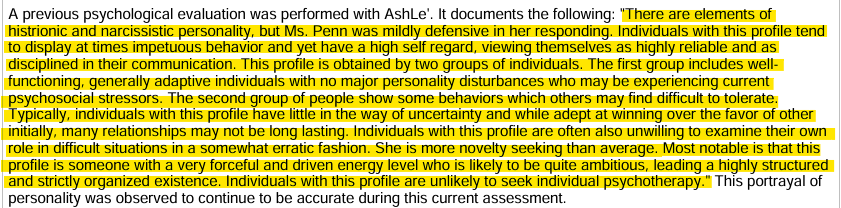
\includegraphics[width=0.78\textwidth]{DHS_Fact_Finding.png}}\\[3pt]
	{\footnotesize\textbf{DHS Fact Finding}}\par
	\vspace{6pt}{\Huge$\updownarrow$}\par\vspace{6pt}
	{\footnotesize\textbf{Full Cited Text}}\par
	\hlbox{\includegraphics[width=0.55\textwidth]{AP_neuro.png}}\\[3pt]
	{\footnotesize\textbf{The record --- Neuropsychological Evaluation}}
	
	{\footnotesize\itshape \emph{The agency's version (top) versus the record (bottom).} At the
		October 31, 2025 trial, ODHS testified under oath that I ``did not engage in \textbf{any}''
		of the services the court ordered. Yet its own Fact Finding (top) quotes the neuropsychological
		evaluation I completed (bottom)---which it possessed, relied upon, and then denied under oath---
		while omitting that same evaluation's findings of no deficits, no clinical diagnosis, no need
		for parenting classes or mental-health treatment, and that ``item endorsement did not indicate
		that Ms.~Penn is at risk of harming her child.''\footnote{A historical unwillingness to engage
			is not sufficient to establish a \textit{current}, non-speculative, serious threat of harm
			likely to be realized.}}
\end{center}

\legalsubsubsection{Selective Use of the Same Evidence --- Mother Framed as Both Irrelevant and Controlling.}

ODHS characterized Mother as ``not playing an active parenting role'' and therefore not disciplining the children.\footnote{Fact Findings Report, pp.~71, 102. } Yet the same report records that ``[t]he girls are doing exactly what she tells them to do'' and that they ``undermine Alquan's authority as a parent.'' \emph{Id.} p.~48. These statements are not necessarily mutually exclusive; a parent may exercise influence without being the day-to-day custodial parent. The problem is that ODHS used the two narratives opportunistically. When minimizing Mother's relationship and parenting capacity, ODHS characterized her as inactive and irrelevant. When attributing conflict, influence, or alleged manipulation to Mother, ODHS characterized her as sufficiently powerful that the children followed her directions over Father's authority. The agency never identified the actual conduct Mother allegedly directed, the context in which it occurred, the source of that assertion, or how that conduct created a current, non-speculative danger to Al-mira. The report uses Mother's alleged influence as adverse evidence while refusing to recognize it as evidence of an active parental bond, parental capacity, or a relationship requiring preservation.

\legalsubsection{Fabricated Third-Party Statements}
\begin{enumerate}
	\item \textbf{Fabricated statement attributed to the maternal grandmother.}\footnote{	2025-11-12 - ODHS Report, p.~23}\\
	Mother's Mother, Marie Penn, has now attested under the penalty of perjury that no such statement was made by her to ODHS. 
	
	
	\begin{center}
		\hlbox{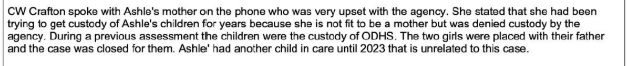
\includegraphics[width=0.78\textwidth]{2025-10-23 - ODHS Report.crafton.marie.png}}\\[3pt]
		{\footnotesize\textbf{ ``CW Crafton spoke with AshLe's mother
				on the phone who was very upset with the agency. She stated that she had been trying to get custody of Ashle's children for years because she is not fit to be a mother but was denied
				custody by the agency.''}}\par\\
	\end{center}
	
	\emph{Contradiction:} The maternal grandmother denies making this statement and so attests by
	signed affidavit.\footnote{Affidavit of Marie A.~Penn (maternal grandmother) available upon request.} Attributing to a named witness a statement she attests that she
	did not make is the \emph{Beltran}/\emph{Spencer} fabrication vector explicitly --- invented witness evidence presented to support removal. This carries no legal protections for ODHS personnel and is a violation the agency is, or should have been well-aware of under the 4th and 14th amendment. 
\end{enumerate}

\legalsubsection{~Fabrications and Internal Contradictions About Mother's Home}

\begin{enumerate}[leftmargin=*,itemsep=0.35em,topsep=0.3em,resume]
	\item \textbf{``Amusement park fun'' \emph{vs.}~``prison.''} Father reports (Fact Findings Report, p.~70): ``amusement park fun.'' Same document, p.~17: A.D.~returned to father's home because she felt Mother's house was a ``prison.''
	\item \textbf{``Homeless'' \emph{vs.}~stable address.} Fact Findings Report, p.~96 (``homeless''); p.~133 (address of record 17548 NW Springville Rd~Apt~9); p.~58 (``resides close to the family'').
	\item \textbf{``In hiding'' \emph{vs.}~``constantly showing up.''} Fact Findings Report, pp.~24, 142 (in hiding); p.~143 (constantly showing up).
	\item \textbf{``Little to no discipline'' \emph{vs.}~directive.} Fact Findings Report, p.~45 (permissive) \emph{vs.}~p.~48 (``girls are doing exactly what she tells them to do'').
\end{enumerate}

\legalsubsection{~Fabrications About Mother's Presence at Father's Home}

\begin{enumerate}[leftmargin=*,itemsep=0.35em,topsep=0.3em,resume]
	\item \textbf{Fact Findings Report, pp.~47, 72, 74:} Mother ``shows up sporadically'' and ``taking the children without permission.'' 2025-10-23 ODHS Report, p.~28: ``Mother is using their father's home as a punishment.''\\
	
	\emph{Contradiction --- Father's own letter to Mother, January 15, 2023 (Exhibit B):} ``Goal with this meeting is for the two of us to work together and co-parent.'' Father set behavioral guidelines for Mother's visits: ``Be respectful of my apartment.\ Clean up after yourself''; ``Don't bring food when the kids tell you they are hungry\ldots\ I would prefer that you come over and teach them how to cook''; ``Stick to your word\ldots''; ``Per our agreement I need you to get the girls on the weekend, NO excuses''; ``DO NOT overstay your welcome. Unless you have spoken with me about spending the night, when I tell you it is time to go, please respect that and leave.''
	
	The letter \emph{invites} and \emph{regulates} Mother's presence at Father's home. It does not prohibit it. The agency has never presented this letter to the court.
	
	\item \textbf{Internal contradiction:} Father simultaneously described as wanting more contact and as the victim of unauthorized contact. Fact Findings Report, p.~47 (``he wants the girls to see their mom more often because `she's their mom'\,'') \emph{vs.}~p.~47 (``Ashle will sometimes `just show up'\,'').
	
	\item \textbf{Independent screener and law-enforcement contradiction.} Fact Findings Report, p.~197: ``reporter is not aware of any no contact order etc that would suggest there would be a legal issue with allowing Ashle inside of the home.'' Same document, p.~181: ``police would not forcibly remove the children from her.''
\end{enumerate}

\legalsubsection{~Fabrication of ``Unwilling or Unable to Protect'' from Father}

\begin{enumerate}[leftmargin=*,itemsep=0.35em,topsep=0.3em,resume]
	\item \textbf{Jurisdictional Allegation B (proven 10/31/2025):} ``The mother fails to recognize the safety threats presents by the father and is unwilling or unable to protect the child from father's unsafe behaviors.''\\
	
	\emph{Direct causation contradiction:} In April 2024, an ODHS worker transported A.D.~from grand jury proceedings directly to Mother's home. ODHS itself then took the position that Al-Quan ``was a safe placement'' and moved to remove the no-contact order --- restoring Father's contact with A.D. Approximately five months later, on September 6, 2025, Father was arrested at his home for Criminal Mischief in the First Degree and Strangulation of A.D. \textbf{The Department cannot allege that I am ``unwilling or unable'' to protect A.D.~from a father whom the Department itself endorsed as a safe placement.}
\end{enumerate}

\legalsubsection{~Fabrication and Concealment of the September 6, 2025 Recantation}

\begin{enumerate}[leftmargin=*,itemsep=0.35em,topsep=0.3em,resume]
	\item \textbf{The 19-minute reversal without disclosure of the same-day recantation.} Kitto text 5:40 PM: ``we can release custody to you.'' Kitto text 5:59 PM: ``suicidal intent if she was made to return to your care.'' Hospital social worker Leah Sathrum documented the statement ``was definitely not what child said initially and worried the change in statements was due to parents' reaction'' (2025-10-13 ODHS Report). \textbf{You yourself acknowledged the recantation on our January 28, 2026 recorded call} at transcript time 19:18 (``once there was a recantation for that to be considered'') and 20:08 (``even given the recantation''). You also said: ``we didn't actually look at mom's parental capacity'' and ``we really don't have any instances of her acting dangerously with regard to the safety of this girl.'' The recantation appears \emph{nowhere} in the September 8, 2025 shelter petition, the September 8, 2025 shelter order, or the diligent-efforts submissions.
\end{enumerate}

\legalsubsection{~Fabrications in the Diligent-Efforts Sworn Submissions}

\begin{enumerate}[leftmargin=*,itemsep=0.35em,topsep=0.3em,resume]
	\item \textbf{Rylan Duffy \emph{Declaration of Diligent Efforts toward Service} (10/10/2025) and Kayla Miller \emph{Affidavit Regarding Efforts to Serve Parent} (10/28/2025)} omit five known channels of contemporaneous contact:
	
	\begin{enumerate}[label=(\alph*),leftmargin=1.5em]
		\item Mother's September 8, 2025 1:44 PM written filing received by the Washington County juvenile clerk;
		\item Clerk Kimberly A.~Beck's September 9, 2025 3:09 PM email acknowledging receipt of the filing;
		\item Mother's September 8, 2025 3:34 PM email to Supervisor Kitto: ``I was effectively prevented from participating by the clerk who refused to assist me in receiving this submission for the shelter hearing'';
		\item Mother's telephonic contact with the juvenile court during the shelter hearing (``Apparently, Mom is called into the court, not to the court hearing'');
		\item The text and email channels through which ODHS itself had communicated with Mother on September 6, 7, and 8, 2025.
	\end{enumerate}
	
	Omission of five known channels of contemporaneous contact from sworn diligent-efforts submissions --- while representing to a court that a parent could not be located --- is judicial deception under \emph{Hardwick v.~County of Orange}, 844 F.3d 1112, 1116--17 (9th Cir.~2017), and warrants review under ORS 162.065 (Perjury) and ORS 162.075 (False Swearing).
\end{enumerate}

\legalsubsection{~Fabrications About the Visitation Record}

\begin{enumerate}[leftmargin=*,itemsep=0.35em,topsep=0.3em,resume]
	\item \textbf{Zero visits.}\footnote{2026-02-23 Review Judgment, p.~3; 2026-06-29 Permanency Judgment, p.~5; 2026-06-18 ODHS Report, p.~8.}
	
	\exfig{0.8\textwidth}{ConsistentVisitation.png}{ODHS's own record of Mother's consistent visitation---contradicting Marquand's testimony that Mother did not complete "any services". \textit{(Source: ODHS visit notes.)}}\\
	
	Marquand would also testify that zero visits have taken place throughout Al-mira's removal from Mother, but the agency was aware at the time the statement was made that this was not true \textit{and} that permanency worker had made statements to the contrary regarding Mother having "done Al-mira's hair" and without any assistance from the agency in reaching her AL-mira thirty miles away. 
	
	\emph{Contradiction 1 --- no visitation plan ever provided:} Penn Supplement, p.~4 (``No visitation plan has been provided to Mother. The agency's failure to provide any assistance while claiming "zero visits have occurred in ten months'' and then attributing the lack of visitation on Mother while the agency is required to provide such service is far from reasonable with regard to the agency's efforts). \emph{Contradiction 2 --- contact restricted without court authorization:} Kitto text of September 7, 2025 at 10:50 AM imposed a contact restriction before any court order authorized restriction. No detriment finding under ORS 419B.090(3) has been made. \emph{Contradiction 3:} 2026-06-18 ODHS Report simultaneously states ``0'' family time visits with Ashle Penn on p.~5 \emph{and} ``Mom has visited with Almira twice'' on p.~5.
\end{enumerate}

\legalsubsection{~Fabrication About the Child's Preference}

\begin{enumerate}[leftmargin=*,itemsep=0.35em,topsep=0.3em,resume]
	\item \textbf{2026-02-12 ODHS Report, p.~30 (Hopkins 90-day staffing note, 1/26/2026):} ``Almira does not want to go to mom --- just wants to be with dad.''
	
	\emph{Contradiction --- Marquand's own sworn testimony 10/31/2025:} Timecode 20:14--20:36: ``she has also said that she will go live with her mother but wants to do family counseling first before that\ldots\ but the child is willing and wanting to engage in that service.'' \emph{Contradiction --- A.D.~directly:} 2025-09-08 Protective Custody Report, p.~6: ``if she couldn't go home to her dad she wanted to go home with her mom.''
\end{enumerate}

\legalsubsection{~Fabrication About the ``Criminal Activities'' Allegation}

\begin{enumerate}[leftmargin=*,itemsep=0.35em,topsep=0.3em,resume]
	\item \textbf{Jurisdictional Allegation C (proven 10/31/2025):} ``The mother is involved in criminal activities which interfere with her ability to safely parent the child.''
	
	\emph{Marquand's own sworn admission (Timecode 13:35--13:44):} ``the agency has not had meaningful contact with the mother to fully assess her and get information about her substance use.'' \textbf{The Department obtained jurisdiction on an unassessed inference.} This fails the standard of \emph{Dep't of Human Servs.~v.~A.W.}, 276 Or~App 276, 278 (2016), requiring a ``current, non-speculative threat of serious loss or injury that is likely to be realized.''
\end{enumerate}

\legalsubsection{~Fabrication About the ``Refused DV Grant''}

\begin{enumerate}[leftmargin=*,itemsep=0.35em,topsep=0.3em,resume]
	\item \textbf{Historical assertion carried into current risk narrative:} Mother refused a DV grant.\\
	
	\emph{Contradiction:} Milne First Call transcript, p.~2--3: ``I went and initiated that DV grant on my own\ldots\ It was never offered to me, nor did I refuse it.'' ODHS records confirm: ``Al Quan will not be receiving the DV grant as Ashle has applied for and received one recently'' (2025-10-07 ODHS Report, p.~131).
\end{enumerate}

\legalsubsection{~Fabrication Regarding Mother's Access to the Case File}

\begin{enumerate}[leftmargin=*,itemsep=0.35em,topsep=0.3em,resume]
	\item \textbf{Implicit representation that ODHS has adequately served Mother with case information.}\\
	
	\emph{Contradiction:} I submitted a formal records request in May 2025 --- five months before removal (2025-10-07 ODHS Report, p.~14). It has not been fulfilled. Judge Rini conditioned my inspection on physical appearance at the Washington County courthouse --- exposing me to arrest on an unrelated warrant I am constitutionally contesting. I obtained the case record only when Al-mira's attorney provided her a zip drive that she delivered to me. I learned the pleaded allegations only when you read them to me on a recorded call.
\end{enumerate}

\legalsubsection{~Fabrications About the September 8, 2025 Clerk Rejection and Service}

\begin{enumerate}[leftmargin=*,itemsep=0.35em,topsep=0.3em,resume]
	\item \textbf{Fabrication that my failure to appear at the shelter hearing was voluntary and appropriately treated as default.}\\
	
	\emph{Contradiction:} I filed a timely written special appearance at 1:44 PM on September 8, 2025 --- before the shelter hearing concluded. The filing was received by the clerk, not docketed, and rejected the next day by Clerk Beck without citation to any statute or rule. The clerk's office subsequently accepted a substantively identical filing (Initial Rejected Filing, pp.~13, 29). I telephonically contacted the court during the shelter hearing itself, as the transcript records: ``Apparently, Mom is called into the court, not to the court hearing.'' No Webex link was provided to me despite Washington County Presiding Judge Order No.~343 mandating Webex generation for all hearings.\\
	
	\item \textbf{Jurisdiction was taken without service of summons.} ``A court may make an order establishing jurisdiction *** only after service of summons.'' ORS 419B.815(1). The first attempt to serve Mother occurred October~14, 2025 --- after the September~8 shelter hearing --- and on that same date Judge Rini stated on the record that ``mom still has not been served,'' which AAG Wadia confirmed. Milne acknowledged the service defect on recorded calls of December~8 and December~25, 2025 (``I want to accept service. I have never evaded service.'').
\end{enumerate}

\legalsubsection{~Emilie Marquand's Sworn Testimony (October 31, 2025 Trial)}

\begin{enumerate}[leftmargin=*,itemsep=0.35em,topsep=0.3em,resume]
	\item \textbf{Sworn witness-tampering allegation delivered without foundation.} \emph{Marquand, Timecodes 6:56--7:05 and 9:56--10:04:} ``There is significant concern that the mother did coach the child to recant these statements after the conversation that the mother had with the child via phone\ldots\ The agency does have concerns that the mother has coached this child. There has been ongoing concerns over the years related to that.''\\
	
	\emph{Contradiction:} No agency record contains any evidence --- no witness statement, no recording, no independent observation --- that Mother coached A.D. Hospital social worker Sathrum's own case note documents the recantation as her contemporaneous observation; her speculative note about ``parents' reaction'' is not a finding of coaching. Marquand's sworn assertion delivered under oath without foundation, and repeated as ``ongoing concerns over the years'' without supporting record, is the \emph{Beltran} fabrication vector: a social worker delivering unsupported speculation as sworn fact. The coaching theory is impossible on the agency's own timeline. ODHS recorded at 2:30~PM on September~6, 2025 that hospital staff had raised a concern about Al-mira recanting based on what Mother would say --- yet Mother's first contact with the child did not occur until approximately 5:00~PM that day, roughly two and one-half hours later. The agency documented a coaching concern before any communication existed through which Mother could have coached. A concern that predates the only conduct that could have caused it is not evidence of that conduct; it is fabrication.%\footnote{\textit{Record cite (Mother to confirm exact page):} ODHS Report documenting the 2:30~PM September~6, 2025 hospital-staff note; Mother's first contact with the child occurred at approximately 5:00~PM September~6, 2025.}
	
	\item \textbf{Sworn testimony contradicted by the same witness thirty seconds later.} \emph{Marquand, Timecode 7:53--8:05:} ``the mother did not engage in any services and actually failed to do any of the services.'' \emph{Marquand, Timecode 12:37--12:41 (same witness, same trial):} ``The mother has engaged in those assessments. The mother has, I will say limitedly, has engaged in those assessments.''
	
	\item \textbf{Marquand's testimony that ODHS ``motioned to dismiss the case'' undermines the ``no engagement'' claim.} Marquand, Timecode 8:41--8:54: ``the agency petitioned or motioned to dismiss the case.'' Agencies do not move to dismiss where a parent has completed nothing. The agency is the custodian of records which contain substantial evidence to the contrary. 
	
	\exfig{0.8\textwidth}{ConsistentVisitation.png}{ODHS's own prior-case visitation record documenting Mother's consistent visitation. This directly contradicts Marquand's sworn testimony that Mother did not engage in \emph{any} services during the prior dependency case. \textit{(Source: ODHS visit notes.)}}
	
	\item \textbf{False ``32 calls'' testimony offered as proof of parental deficiency.} Marquand --- a caseworker of eight and one-half years, required to review a family's prior child-welfare history --- testified that ``32 calls'' were logged under Mother, ``19 of those calls being assigned for assessment,'' and ``20 calls'' under Father, ``10 of which have been assigned,'' and presented the count as proof that Mother ``does not understand'' her child's needs and ``lacks skills.''\footnote{Marquand testimony, Timecodes 7:24--7:31, 11:17--11:31.} The count proves no such thing, and the agency's own intake history --- which Marquand was obligated to read --- establishes that it does not. Of the nineteen reports screened in under Mother's case between 2011 and 2025, the \textbf{sole} founded allegation against Mother is a single 2019 Threat of Harm --- a \emph{failure to protect} her children from the domestic violence of Barry Washington (whom the agency's own report elsewhere miscalls ``Barry Sanders''). That finding is six years old, arose from a third party's violence, and issued without the founded-disposition letter that would have allowed Mother to challenge it. The finding is not evidence of abuse or neglect by Mother in any event: the agency's own narrative founds it because Mother ``refused to cooperate with the district attorney's office when charges were filed against'' her abuser for strangulation, and because she obtained and then dismissed restraining orders against him. It founds a domestic-violence survivor for her abuser's violence and for declining to assist his prosecution. A survivor's response to her own abuser is not a parenting deficiency, and the agency's failure to send the mandatory founded-disposition notice left even this finding insulated from the challenge Mother was entitled to bring. Every other screened-in report closed \emph{unfounded} or \emph{unable to determine}; the present case is \emph{pending}. No substance-abuse allegation appears anywhere in the history --- the ``substance abuser'' label originated as Father's uncorroborated report. Father's own case carries a nearly identical volume (nineteen reports, nine screened in), confirming the count reflects a high-conflict household and the agency's practice of filing every report under the mother's name, not a deficiency in Mother. A tally of contacts is not a finding, and it cannot establish the present, non-speculative danger jurisdiction requires. \emph{A.\,W.}, 276 Or App at 278.
	\begin{center}\footnotesize
		\begin{tabular}{@{}lcc@{}}
			\hline
			\textbf{Agency intake history (CF307A)} & \textbf{Mother (Penn)} & \textbf{Father (Davis)} \\ \hline
			Total reports, 2011--2025 & 32 & 19 \\
			Screened in for assessment & 19 & 9 \\
			Closed at screening & 13 & 10 \\
			Founded against the parent & 1 (2019 failure-to-protect) & --- \\
			Substance-abuse allegations & 0 & --- \\ \hline
		\end{tabular}
	\end{center}
	
	\exfig{0.9\textwidth}{SOLEFOUNDEDALLEGATION.png}{The agency's own Fact Findings narrative: the sole Threat-of-Harm finding coded against Mother is a \emph{failure to protect} her children from the ``significant pattern of domestic violence'' perpetrated by Barry Washington --- a past finding arising from a third party's violence, not from any act of Mother's. \textit{(Source: 2025-09-08 Fact Findings Report.)}}
	
	\exfig{0.85\textwidth}{CallsHistory_1.png}{The agency's own CPS intake table (form CF307A). Each report shows its Screening Decision and Case Name --- reports under ``Penn, Ashle'' are Mother's; those under ``Davis, Alquan'' are Father's. \textit{(Source: 2025-09-08 Fact Findings Report, CF307A.)}}
	
	\exfig{0.85\textwidth}{CallsHistory_2.png}{Continuation of the CF307A intake table: the founded dispositions cluster in 2019 and name Barry Washington; the remaining assessments close unfounded or unable to determine. \textit{(Source: 2025-09-08 Fact Findings Report, CF307A.)}}
	
	\item \textbf{False ``refused to pick up the child'' testimony.} Marquand testified that Mother ``refused to pick this child up from the hospital.'' The agency's own Protective Custody Report records the opposite: Mother ``was finally able to be reached at 4:31pm and indicated that she was in the community and couldn't get to the hospital except by bus and that would be several hours,'' that she ``couldn't get the time off work like she thought she could \emph{but was sending the uncle instead},'' and that worker Bennett ``attempted to make plans to meet with and transport Ashle to her daughter.'' The uncle Mother sent was certified by the agency as the child's relative placement within twenty-four hours. Mother did not refuse; she arranged the relative resource the agency then approved. The agency omitted each of these facts from its testimony to the court.
	
	\item \textbf{Inaccurate sworn testimony about Mother's warrants, confirming the absence of firsthand knowledge.} Marquand testified that Mother ``failed to appear to her hearing on June 23 of 2025 for the theft of the first degree but there was no warrant issued in my understanding for that case,'' attributing the active warrant instead to a separate ``possession of meth and theft'' charge. The law-enforcement record is otherwise: a single felony failure-to-appear warrant issued on the theft-in-the-first-degree and unlawful-possession-of-methamphetamine charges together. Hillsboro Police Dept.\ GO 2025-17657. Marquand's ``in my understanding'' qualifier, and her misdescription of the warrants, confirm she testified from second-hand paperwork she had not accurately reviewed --- the same absence of personal knowledge, OEC 602, that infects her testimony throughout.
	
	\exfig{0.8\textwidth}{GAO_NoLetter.png}{Governor's Advocacy Office (\#34714): no founded-disposition letter against Mother could be located. \textit{(Source: GAO correspondence.)}}
	
	\item \textbf{Sworn fabrication --- the 20 hotline calls / 10 assessments regarding Father's case since 2021.} Marquand, Timecode 11:17--11:31. ODHS did not open a dependency case on Father until the September 6, 2025 assault. The agency's own failure to open a case is not Mother's failure to protect.
	
	\item \textbf{Sworn fabrication --- blaming Mother for not modifying a custody order she was jurisdictionally barred from modifying.} Marquand, Timecode 12:59--13:04. Mother did attempt to modify custody after the April 2024 arraignment; the Washington County court declined jurisdiction on jurisdictional grounds unrelated to Mother.
	
	\item \textbf{Sworn fabrication contradicted by A.D.'s own recorded preference.} Marquand, Timecode 20:14--20:36 (see Item above for the direct contradiction).
\end{enumerate}

\legalsubsection{~Judge Rini's Ordered Services Contradict Dr.~Tongue's Court-Ordered Expert Evaluation}

\begin{enumerate}[leftmargin=*,itemsep=0.35em,topsep=0.3em,resume]
	\item \textbf{Dispositional order requiring Mother to ``participate in parent education classes.''} Judge Rini's disposition order, Timecode 27:29--27:35.
	
	\emph{Contradiction --- Dr.~Tongue's court-ordered evaluation, Recommendation~2:} ``Ms.~Penn, in my opinion, does not merit referral for parent training. She seems to have an adequate understanding of child development and parenting practices which would likely not be improved by attending the typical parenting class.'' Ordering redundant, unnecessary services in direct contradiction of the agency's expert violates ORS 419B.343(1)(a), which requires ordered services to be ``rationally related to the jurisdictional findings.'' Under OEC 702--703, a social-worker lay opinion cannot substitute for a psychologist's controlled clinical testing.
\end{enumerate}

\legalsubsection{~Judicial Misleading Characterization of Mother's Habeas Filing}

\begin{enumerate}[leftmargin=*,itemsep=0.35em,topsep=0.3em,resume]
	\item \textbf{Judge Rini's ruling, Timecode 16:33--16:52:} ``Ms.~Penn has attempted to file habeas corpus motions to get him out of custody.''
	
	\emph{Contradiction:} The judge cited no source. The actual predicate: Washington County Sheriff's deputies entered Mother's home based on an administrative order signed by a Washington County Community Corrections officer --- not a judicial warrant. Deputies did not have consent to enter. The State could not produce the document at the time of arrest. The State produced an ``order of arrest'' only 73 days later, signed by a person laid off shortly thereafter and whom the State refused to call as a witness. The habeas filing raised the Fourth Amendment violation of Mother's own home. To describe it as an attempt to ``get him out of custody'' strips the Fourth Amendment predicate and imports an association-based innuendo.
	
	\emph{Independent corroboration of the retaliatory posture --- Washington County HR (Exhibit K):} September 19, 2025 fee-waiver denial letter from Aaron Mendes cites --- as Ground (c) --- the County's belief that Mother intends to ``provide legal assistance to the \textless\textless convicted\textgreater\textgreater\ perpetrator of the crimes she is the victim of.'' That admission on the face of the County's own denial confirms that Mother's constitutionally protected legal activity is being used against her across at least two county departments.
\end{enumerate}

\bigskip

\begin{center}
	\rule{0.5\textwidth}{0.4pt}
\end{center}

\bigskip

\legalsection{Neither Absolute Nor Qualified Immunity Shields This Conduct}
The Ninth Circuit forecloses \emph{both} forms of immunity for the conduct documented
here. \textbf{Absolute immunity} does not apply: social workers may enjoy it when
performing functions ``critical to the judicial process itself,'' but they are ``not
entitled to absolute immunity from claims that they fabricated evidence during an
investigation or made false statements in a dependency petition,'' because such acts
``aren't similar to discretionary decisions about whether to prosecute.'' \textit{Beltran
	v.~Santa Clara County}, 514 F.3d 906, 908 (9th Cir.~2008) (en banc).

\textbf{Qualified immunity} does not apply either, because the right at issue was clearly established years
before this case. Sitting en banc in \textit{Devereaux v.~Abbey}, 263 F.3d 1070, 1074--75
(9th Cir.~2001), the court held that ``there is a clearly established constitutional due
process right not to be subjected to criminal charges on the basis of false evidence that
was deliberately fabricated by the government,'' adding that ``[a]nyone who acts on behalf
of the government should know that a person has a constitutional right not to be
`framed.''' The court extended that rule to the civil child-welfare context in
\emph{Costanich v.~Department of Social \& Health Services}, 627 F.3d 1101, 1108 (9th
Cir.~2010), holding that ``deliberately fabricating evidence in civil child abuse
proceedings violates the Due Process [Clause] of the Fourteenth Amendment,'' and that the
right is ``sufficiently obvious'' to deny a social worker qualified immunity. Deliberate
fabrication may be proven by circumstantial evidence. \emph{Spencer v.~Krause}, 857 F.3d
789 (9th Cir.~2017).\\

\textbf{The pattern is not confined to ODHS, and it is not a single mistake.} Twice, in two counties, the agency has placed a fabricated characterization of Mother before a court while its own contemporaneous records established the truth: in 2020, ODHS told the Multnomah County court that Mother thought herself ``too good'' for a shelter the day after its own family-planning notes recorded that Mother had pursued that very resource and been told she was ineligible (Figures above); and in 2025, ODHS built the present case on the fabrications and omissions catalogued here. Washington County Human Resources (Exhibit K) and the Washington County District Attorney (Exhibit L) have each adopted the same retaliatory posture, using Mother's constitutionally protected legal activity against her. A local government is liable under 42 U.S.C. § 1983 where a policy, custom, or persistent practice causes the constitutional injury, \emph{Monell v.~Dep't of Social Servs.}, 436 U.S. 658, 690--91 (1978), and it enjoys no qualified immunity for such a claim, \emph{Owen v.~City of Independence}, 445 U.S. 622 (1980). The cross-county, cross-department pattern documented here is the custom that Monell reaches, and it forecloses any good-faith-mistake defense.\\

\textbf{The Pattern Extends Beyond ODHS}

The fabrication and retaliation pattern documented above is not confined to ODHS. Washington County Human Resources (Exhibit K) has denied fee waivers on the basis of Mother's constitutionally protected legal activity. Washington County District Attorney (Exhibit L) has, on appeal, adopted the same view. Judge Rini has imported that view onto the record of the dependency proceeding through the habeas mischaracterization above. A supervisor with knowledge of a cross-department retaliation pattern cannot claim, in good faith, that the record reflects a good-faith mistake.

\bigskip

The record above is not a series of isolated errors. The agency's diligent-efforts certification omitted mother's still pending objection to referee jurisdiction. Without the court having identified lawful basis for rejecting Mother's submission, the court clerk had no authority to reject it. The agency's ``no relative available'' posture at removal is refuted by the agency's own certification of the maternal relative provided by mother, prior to protective custody being taken, as placement within twenty-four hours. The agency's ``unwilling to engage'' characterization is refuted by the agency's own notes recording mother's arrangement of this family presence and her direction of communication to a supervisor in writing. The agency's coaching allegation is temporally impossible on the agency's own contact log. The agency's finding that mother ``does not understand'' her child's needs was rendered by a witness who is not clinically credentialed to make that finding and who ignored a licensed neuropsychologist's contrary evaluation of the same capacity while claiming the very record quoted and mischaracterized didn't exist. The agency restricted the child's disclosure to her mother, and suspended mother's contact with her child, without a court order authorizing either restriction. \textbf{The agency's shelter presentation substituted 285 pages of historical case material, or material directly related to father's incident which caused Al-mira's entry into care, for the present-danger predicate ORS 419B.180 requires.} Each defect is documented in the file. Amelioration and restorative actions are, at this juncture, not discretionary.

\exfig{0.45\textwidth}{VisitsGoWell.png}{ODHS's own note that visits went well---contradicting the ``zero visits'' entries in the judgments.}\footnote{ODHS visit notes.}

\textbf{What Your Commitment Now Requires}

Consistent with your January 28, 2026 recorded standard, I request that within \textbf{seventy-two (72) hours} of receipt of this letter you:

\begin{enumerate}[leftmargin=*,itemsep=0.25em]
	\item Review Exhibits A through S and this case's full record;
	\item Produce a written determination, addressed to me, identifying each representation catalogued above that ODHS now concedes to be false, unsupported, or materially incomplete, and identifying each that ODHS maintains, with the record citation on which it relies;
	\item Correct the record before the juvenile court, as you committed on January~28, 2026 to do upon finding perjured or concerning information, by filing a written notice of correction that discloses the recantation withheld from the September~8, 2025 shelter hearing, the diligent-efforts omissions, and the fabricated statements attributed to Mother and to the maternal grandmother;
	\item Join Mother's motion under ORS 419B.923 to set aside the October~31, 2025 default and the judgments that rest on it, or file a statement of non-opposition to that motion;
	\item Refer Emilie Marquand, and the authors of the sworn diligent-efforts submissions, for review under ORS 162.065 (Perjury) and ORS 162.075 (False Swearing), and for professional-conduct review;
	\item Provide Mother a concrete visitation plan and the transportation assistance the agency has withheld, and cease treating Mother's assertion of her constitutional rights as evidence of danger; and
	\item Preserve all records identified in this letter pending resolution.
\end{enumerate}

\legalsection{Preservation of Evidence}
This letter, its exhibits, and the recorded calls of January~28, 2026 and April~28, 2026 place ODHS on notice of pending and anticipated litigation. ODHS, its counsel, and each recipient shall preserve all records, communications, case notes, drafts, metadata, recordings, and electronically stored information relating to \textit{In re A.D.}, No.~25JU04261, and to Mother's prior involvement with the agency. The duty to preserve extends to text messages, emails, CF307A intake records, screening decisions, and the diligent-efforts file. Destruction or alteration of these records after receipt of this notice supports an adverse inference and sanctions.

\legalsection{Reservation of Rights}
Nothing in this letter waives any right, claim, or remedy. Mother reserves all claims under 42 U.S.C. § 1983, the Oregon Tort Claims Act, and Oregon law, and all rights to move to set aside the judgments entered without service, to seek review of the orders that rest on the default, and to pursue the oversight avenues identified in the copy list. This letter is written notice under your recorded commitment; it is not the limit of the relief Mother will seek if the record is not corrected.

\begin{center}
	\rule{0.5\textwidth}{0.4pt}
\end{center}

\vspace{0.5em}
Ms.~Faulkner, you told me on a recorded line that if you found perjury or unlawful conduct in this record, you would ``absolutely handle that'' with your employees and ``notify the court.'' The record is now in front of you. What you do with it is the measure of that commitment.

\vspace{1.5em}
\raggedright
Respectfully,\\[2.5em]
/s/ \includegraphics
AshLe' Antoinette Penn\\
\textit{Mother, self-represented}\\
17548 NW Springville Road, Unit 9\\
Portland, OR 97229\\
(424) 242-3374 \textbullet\ ashlepenn.ap3@gmail.com

\vfill
\begin{center}
	{\color{steel}\rule{\textwidth}{0.4pt}}\\[3pt]
	{\footnotesize\color{steel}\textit{Appendix A --- Proposed Stipulation --- follows.}}
\end{center}

\clearpage
\legalsection{Appendix A --- Proposed Stipulation and Order}
\textit{Mother offers the following stipulation to resolve the record defects identified above without the need for contested litigation of the threshold jurisdictional question. Mother's offer of this stipulation is not a concession of any fact and preserves every right reserved above.}

\vspace{0.75em}
\textbf{Recitals.}
\begin{enumerate}[label=\Alph*., leftmargin=*,itemsep=0.35em]
	\item A juvenile court may make an order establishing jurisdiction only after service of summons. ORS 419B.815(1).
	\item The agency's Declaration of Diligent Efforts (Duffy, Oct.~2025) and Affidavit Regarding Efforts to Serve Parent (Miller, Oct.~2025) state that service was not accomplished by personal, substituted, office, or mail service.
	\item The agency's own diligent-efforts file returned Mother's current address, 17548 NW Springville Rd., \#9, from CLEAR, Accurint, Medicaid, and Mother's open TANF case, and Mother's family coach confirmed that address on October~13, 2025.
	\item Mother communicated with the agency by telephone and email during September and October 2025, and filed written submissions with the juvenile court on September~8, 2025.
	\item The court found Mother in default under ORS 419B.914 on October~31, 2025, a statute that permits proceeding without service only where diligent efforts fail to reveal the parent's whereabouts.
	\item The self-harm statement that drove the September~6, 2025 protective custody was recanted the same day, was documented by the agency, and does not appear in the September~8, 2025 shelter petition or order.
	\item The Citizen Review Board review in No.~25JU04261 remains pending.
\end{enumerate}

\vspace{0.5em}
\textbf{Stipulated Terms.}
\begin{enumerate}[label=\arabic*., leftmargin=*,itemsep=0.35em]
	\item ODHS shall join, or file a statement of non-opposition to, Mother's motion under ORS 419B.923 to set aside the October~31, 2025 order finding Mother in default and the jurisdictional, dispositional, review, and permanency judgments that rest upon it.
	\item Upon the setting aside of the default, ODHS shall complete service of summons by a method authorized under ORS 419B.823 or 419B.824, or move for court-ordered alternative service, so that any jurisdictional determination proceeds on proper notice and a contested record.
	\item ODHS shall file a written correction of the record disclosing the September~6, 2025 recantation, the diligent-efforts omissions, and the statements attributed to Mother and to the maternal grandmother that each denies.
	\item Pending resolution, ODHS shall provide Mother a written visitation plan and reasonable transportation assistance, and shall not treat Mother's assertion of her constitutional rights as evidence of danger.
\end{enumerate}

\vspace{2em}
\raggedright
\begin{minipage}{0.45\textwidth}
	\rule{\linewidth}{0.4pt}\\
	Sonya Faulkner, D16 Manager, ODHS\\
	Date: \underline{\hspace{2in}}
\end{minipage}
\hfill
\begin{minipage}{0.45\textwidth}
	\rule{\linewidth}{0.4pt}\\
	AshLe' Antoinette Penn, Mother\\
	Date: \underline{\hspace{2in}}
\end{minipage}

\end{document}